%\documentclass{beamer}

\documentclass[10pt]{beamer}
\usepackage{pgfpages}
%\usepackage{Sweave}
\usepackage{graphicx, overpic}
%\DeclareGraphicsExtensions{.pdf,.png,.jpg}
\usepackage[english]{babel}
\usepackage{amsmath}
\usepackage{enumitem}
\usepackage{fancyvrb}
\usepackage[utf8]{inputenc}
\usepackage{listings}
\usepackage{tabularx}
\usepackage{tikz,url,ragged2e}
%\usepackage{auto-pst-pdf}
\usetikzlibrary{calc}
\usepackage{pstricks,pst-node,pst-text,pst-3d,graphicx,hyperref,color,epsfig,bm,pifont,xspace}
%\usefonttheme[onlymath]{serif}
%\usepackage{appendixnumberbeamer}

%\usepackage{pgfpages}
%\pgfpagesuselayout{resize to}[a4paper,border shrink=5mm,landscape]

%%%%% UNCOMMENT THIS TO PRODUCE HANDOUTS %%%%
% NB add option handout to the documentclass
%\usepackage{handoutWithNotes,pgf,pgfpages}
%\pgfpagesuselayout{3 on 1 with notes}[a4paper,border shrink=5mm]
%%%%%%%%%%%%%%%%%%%%%%%%%%%%%%%%%%%%%%%%%%%%%

\mode<presentation>{\usetheme{Boadilla}}
\setbeamertemplate{itemize item}{$\bullet$} %
\setbeamertemplate{itemize subitem}{--} %
\setbeamertemplate{itemize subsubitem}[circle] %
\setbeamertemplate{navigation symbols}{}

\newrgbcolor{myblue}{0.14 0.34 0.55}
\newrgbcolor{orange}{1 0.5 0}
\newrgbcolor{olive}{.2 .31 .09} %%% 52 .61 .15
\newcommand{\pb}[1]{\parbox[c][.3cm][c]{.3cm}{\centering#1}}
\newcommand{\pd}[1]{\parbox[c]{.4cm}{\centering#1}}
\newcommand{\mytilde}{{\raise.17ex\hbox{$\scriptstyle\mathtt{\sim}$}}\xspace}

\def\colorize<#1>{%
\temporal<#1>{\color{black!10}}{\color[rgb]{0.14,0.34,0.55}}{\color{black!35}}}


\newcommand\ex[1]{{\small{\color{teal}{#1}}}}
\setbeamersize{text margin left=0.5cm,text margin right=0.5cm}
\setbeamercolor{equation.box}{fg=blue,bg=yellow!50!white} \setbeamercolor{postit}{fg=black,bg=yellow!75!white}
\setbeamertemplate{navigation symbols}{}
\DefineVerbatimEnvironment{ColorVerbatim}{Verbatim}%
  {formatcom=\color{black},commandchars=\\\{\}}
 
  
\setbeamertemplate{footline}
{
  \leavevmode%
  \hbox{%
  \begin{beamercolorbox}[wd=.4\paperwidth,ht=2.25ex,dp=1ex,center]{author in head/foot}%
    \usebeamerfont{author in head/foot}\insertshortauthor
  \end{beamercolorbox}%
  \begin{beamercolorbox}[wd=.6\paperwidth,ht=2.25ex,dp=1ex,center]{title in head/foot}%
    \usebeamerfont{title in head/foot}\insertshorttitle\hspace*{3em}
    \insertframenumber{} / \inserttotalframenumber\hspace*{1ex}
  \end{beamercolorbox}}%
  \vskip0pt%
}
%%%%%%%%%%%%%%%%%%%%%%%%%%%%%%%%%%%%%%%%%%%%%%%%%  

  

\title[Spatial and Spatio-Temporal Bayesian Models with R-INLA] % Module title to go in the footer on each slide
{\Huge{Spatial and Spatio-Temporal Bayesian Models with R-INLA}}

\author[27 August 2019]{}  % Short lecture title to go in footer on each slide

%\institute[Lecture 2]{}  % Lecture number, to go in footer on each slide

\date[]{}

%\documentclass[handout]{beamer}
%\usepackage{graphicx,hyperref,color,epsfig}
%\usepackage[UKenglish]{babel}
%\usefonttheme[onlymath]{serif}
%
%\mode<presentation>
%%\usetheme{default} %Boadilla Singapore Warsaw
%\usetheme{Boadilla}
%%\setbeamercovered{transparent} %
%\setbeamertemplate{itemize item}{$\bullet$} %
%\setbeamertemplate{itemize subitem}{--} %
%\setbeamertemplate{navigation symbols}{}

%%\title[\fontsize{4}{4} \selectfont MC and WinBUGS]{\fontsize{15}{15} \selectfont Introduction to monte Carlo methods and WinBUGS}
%\date[\fontsize{4}{4} \selectfont Centre for Disease Control]{}
%\author[\fontsize{4}{4} \selectfont Bayesian Analysis of Small Area Health Data]{}
%\title[\fontsize{4}{4} \selectfont WinBUGS and GeoBUGS]{}
%%\institute[\fontsize{4}{4} \selectfont Imperial
%%College]{}
%
\begin{document}
\AtBeginSection[] {
   \begin{frame}
       \frametitle{Outline}
       \tableofcontents[currentsection]
   \end{frame}
}


\AtBeginSubsection[]
{
\begin{frame}<beamer>
\frametitle{Outline}
\tableofcontents[currentsection,currentsubsection]
\end{frame}
}

\begin{frame}[t]
  \titlepage
  \vspace{-2cm}

\begin{tabular}{lll}
\Large{Marta Blangiardo} && \Large{Michela Cameletti}\\ 
&&\\
Imperial College London && University of Bergamo\\
\small{\url{m.blangiardo@imperial.ac.uk}}&&\small{\url{michela.cameletti@unibg.it}}
\end{tabular}

\end{frame}

%%%%%%%%%%%%%%%%%%%%%%%%%%%%%%%%%%%%%%%%%%%%%%%%%%%%%%%%%%%%%%%%%%%%%%%%
%\begin{frame}
%\frametitle{Learning objectives}
%After this lecture you should be able to 
%\begin{itemize}
%\vfill\item Present the class of latent Gaussian models 
%\vfill\item Present the Laplace approximation and the INLA approach
%\vfill\item Use the basic functions of the \texttt{R-INLA} package 
%\end{itemize}
%
%\vfill The topics treated in this lecture are presented in Chapter 4 of the INLA book.
%
%
%\end{frame}
%%%%%%%%%%%%%%%%%%%%%%%%%%%%%%%%%%%%%%%%%%%%%%%%%%%%%%%%%%%%%%%%%%%%%%%%
\begin{frame}
\frametitle{Spatial epidemiology - definition}
\vfill\begin{itemize}
\justifying
\item {\bf Epidemiology}: The study of the distribution, causes and control of diseases in human population.
\item Disease risk depends on the classic epidemiological trio of person (in terms of genetics and behaviour), place and time   [spatial epidemiology focuses on 2 and 3].
\item Place is a surrogate for exposures present at that location, e.g. environmental exposures in water/air/soil, or the lifestyle characteristics of those living in particular areas.
\end{itemize}

\vfill\begin{block}{}
Describing and understanding spatial variation in disease risk and its link with environmental and other potential causes of disease
\end{block}
\end{frame}


%%%%%%%%%%%%%%%%%%%%%%%%%%%%%%%%%%%%%%%%%%%%%%%%%%%%%%%%%%%%%%%%%%%%%%%%
%\subsection[Data]{}


\begin{frame}
    \frametitle{Types of data}
\begin{itemize}
\justifying
 \vfill \item \textbf{Point-referenced data}: the exact location of the case is known
        \begin{itemize}
        \justifying
        \item rarely available routinely, can be collected through case-control studies or specialized survey
        \item if location itself is \emph{random}, e.g. measurements of where events occur\\
         $\Rightarrow$ point process statistical framework
        \item if locations are \emph{fixed} (monitoring stations, postcodes in an area)
         and outcome is measured at each location (e.g. presence/absence of cases, pollution concentrations)\\
         $\Rightarrow$ geostatistical framework.
        \end{itemize}
\pause\vfill  \item \textbf{Area data or count data}: locations are areal units with well defined geographical boundaries, usually administrative units
        \begin{itemize}
        \justifying
        \item outcome is number of cases aggregated over the area (and time)
        \item most common type of data collected.
        \end{itemize}
        \medskip
 \vfill  \item We will concentrate on non-infectious diseases and count data.
\end{itemize}
\end{frame}

%%%%%%%%%%%%%%%%%%%%%%%%%%%%
\begin{frame}
\frametitle{Need for spatial methods}
\begin{itemize}
\justifying
\vfill\item All epidemiological studies are spatial.
\vfill\item Often the study area is small and/or there is abundant individual-level information and so spatial location is not acting as a surrogate for risk factors.
\vfill\item When are we interested in the spatial component?
	\begin{itemize}
	\justifying
	\vfill\item Are we explicitly interested in the spatial pattern of disease risk?\\
	Spatial pattern suggests that observations close to each other have more similar
	values than those far from each other.
	
	$\rightarrow$ disease mapping, cluster detection.
	\vfill\item Is the clustering a nuisance quantity that we wish to take into account but are not explicitly interested in? 
	
	$\rightarrow$ spatial regression.
\end{itemize} 
\end{itemize}
\end{frame}

%%%%%%%%%%%%%%%%%%%%%%%%%%%%%
%\begin{frame}
%    \frametitle{Types of studies with a spatial component}
%\begin{itemize}
%\justifying
%  \item[] \textbf{Disease mapping} 
%  \begin{itemize}
%  \justifying
%  \item spatial and spatio-temporal variation in disease risk
%  \item exploit spatial dependence in order to smooth rates and provide better predictions
%\end{itemize}   
%  \item[] \textbf{Ecological regressions}
%   \begin{itemize}
%   \justifying
%      \item Aim is to examine how geographical variations in health outcomes relate to geographic variations in exposure of interest (e.g. air pollution)
%      \item  Association between risk and exposures at the {\color{red}{area level}}
%      \item Can address aetiological and/or public health questions
%      
%         \end{itemize}
%  \item[]\textbf{Disease clustering and cluster detection}
%    \begin{itemize}
%    \justifying
%      \item Disease clustering: specific patterns of heterogeneity in space\\
%       $\rightarrow$ tendency of disease risk
% \item Cluster detection: identification of unusual aggregations of cases\\
%       $\rightarrow$ reveal hotspots
%    \end{itemize}
%\end{itemize}
%\end{frame}



%%%%%%%%%%%%%%%%%%%%%%%%%%%%
%\section{General framework}
\frame{
\huge \red 
\begin{center}
\textbf{General framework}
\end{center}
}

%%%%%%%%%%%%%%%%%%%%%%%%%%%%


\begin{frame}
    \frametitle{General framework for small area studies - I}
\begin{itemize}
\justifying
\item \textbf{Data} for a region of interest/reference area, geographical level and a specific period

		\uncover<2->{\ex{England, ward level, 2009-2012}}
        \begin{itemize}
            \item $y_i$: Observed number of cases in area $i$\\
				\uncover<3->{\ex{Lung cancer deaths in males aged 45+}}\\
				\uncover<5->{\ex{Congenital anomalies}}\\
            \item $n_i$: Population at risk in area $i$\\
            \uncover<4->{\ex{Male population aged 45+}}\\
            \uncover<6->{\ex{Live births and stillbirths}}\\
        \end{itemize}
\item \textbf{Parameter of interest} Relative risk $\phi_i$ in each area compared with the chosen reference area.
\end{itemize}
\end{frame}


%%%%%%%%%%%%%%%%%%%%%%%%%%%%

\begin{frame}
    \frametitle{General framework for small area studies - II}
\begin{itemize}
\vfill\item Standard statistical model if rare disease and/or small areas
$$y_i \sim \hbox{Poisson}({\color{red}\phi_i} E_i)$$
where $E_i$ = expected nb of cases in area $i$

\vfill

\item ${\color{red}\phi_i}$ estimated by Standardised Mortality/Incidence Ratio (maximum likelihood estimator)\\
\begin{equation*}
\begin{array}{ccc}
\hat{\phi}_i = \hbox{SMR}_i \hbox{ or SIR}_i  =  \frac{y_i}{E_i} & \text{and} &\hbox{Var}(\hat{\phi}_i) =  \frac{\phi_i}{E_i} \rightarrow \hat{\hbox{Var}}(\hat{\phi}) =  \frac{y_i}{E_i^2}
\end{array}
\end{equation*}
\end{itemize}

\vspace{1cm}
\noindent {\small
$\text{Recall: }X \sim \hbox{Poisson}(\mu) \Leftrightarrow \hbox{E}(X) = \hbox{Var}(X)=\mu$
}
\end{frame}

%%%%%%%%%%%%%%%%%%%%%%%%%%%%

\begin{frame}
    \frametitle{Expected numbers of cases - definition}
\begin{itemize}
\justifying
  \item Expected nb of cases if the population had the same stratum-specific mortality/incidence rates as in a reference area.
  \item Adjustments (strata): age, gender, maternal age,...
  
  \end{itemize}

\begin{block}{Indirect standardisation}
    $$E_i = \sum_j n_{ij} r_j$$
with
      \begin{itemize}
      \item[] $r_j$: disease rate for stratum $j$ in the reference population
      \item[] $n_{ij}$: population at risk in area $i$, stratum $j$
      \end{itemize}
\vspace{0.2cm}
If internal comparison: $\sum_{i=1}^N y_i = \sum_{i=1}^N E_i$
\end{block}
\note{
\begin{itemize}
\item age will almost need controlling for since different disease risks in different areas may reflect differences in age population
\item direct standardisation: apply the disease rate in the population of interest (e.g. UK) to a standard population e.g. European standard population
\item external comparison: if the reference population is not the population of the study of interest. For ex, to calculate the expected numbers in London, risks in England could be used
\end{itemize}
 }
\end{frame}
%%%%%%%%%%%%%%%%%%%%%%%%%%%%%%%%%%%%%%%%%%%%%%%%%%%%%%%%%%%%%%%%%%%%%%%%
\begin{frame}
    \frametitle{Lung cancer incidence in males, 1985-2009, England and Wales}
\begin{columns}
    \begin{column}{8cm}
        \begin{center}
        SIRs at ward level
        \scalebox{0.35}{\includegraphics{Figures/Lungmales_SMRmap.jpg}}
        {\tiny
\begin{table}
    \begin{tabular}{|l|l|l|l|l|l|}
        \hline
        ~   & Min  & Q1    & Median & Q3    & Max    \\ \hline
        y   & 0    & 26    & 47     & 84    & 456    \\
        E   & 3.25 & 32.14 & 53.60  & 82.47 & 390.49 \\
        SMR & 0    & 0.70  & 0.89   & 1.13  & 2.63   \\
        \hline
    \end{tabular}
\end{table}
}
\end{center}
    \end{column}
    \begin{column}[c]{4cm}
        \uncover<2->{Is the variability real or simply reflecting unequal $E_i$s?\\
                  \vspace{0.5cm}
        Have the highlighted areas truly a raised relative risk?}
    \end{column}
\end{columns}


\end{frame}
%%%%%%%%%%%%%%%%%%%%%%%%%%%%%%%%%%%%%%%%%%%%%%%%%%%%%%%%%%%%%%%%%%%%%%%%
\begin{frame}
    \frametitle{Problems with mapping SMRs}
\begin{itemize}
\justifying
\vfill\item Common practice is to map SMRs
    \begin{itemize}
    \item[$\rightarrow$] $\hbox{SMR}$ very imprecise for rare diseases and/or areas with small populations
  \item[$\rightarrow$] SMR in each area is estimated independently
    \begin{itemize}
    \item[$\rightarrow$] makes no use of risk estimates in other areas of the map, even though these are likely to be similar.
    \end{itemize}
\vspace{0.2cm}
\pause\item[$\Rightarrow$] Highlights extreme risk estimates based on small numbers.
\vspace{0.2cm}
\item[$\Rightarrow$] Ignores possible spatial correlation between disease risk in nearby areas due to possible dependence on spatially varying risk factors.
\end{itemize}
\end{itemize}
\vfill\pause\color{red}{Problems addressed using Bayesian `smoothing' estimators in a hierarchical formulation}:\\
\begin{itemize}
\item Poisson-logNormal model: non spatial smoothing
\item Poisson-logNormal-spatial model: spatial and non spatial smoothing
\end{itemize}
\end{frame}


%%%%%%%%%%%%%%%%%%%%%%%%%%%%%%%%%%%%%%%%%%%%%%%%%%%%%%%%%%%%%%%%%%%%%%%%
%\section{Bayesian inference}
\frame{
\huge \red 
\begin{center}
\textbf{Bayesian inference}
\end{center}
}
%%%%%%%%%%%%%%%%%%%%%%%%%%%%%%%%%%%%%%%%%%%%%%%%%%%%%%%%%%%%%%%%%%%%%%%%

%\begin{frame}
%    \frametitle{Bayesian thinking}
%    \vspace{-5mm}
%   \begin{center}
%    \scalebox{0.6}{\includegraphics{Figures/Thinking2.pdf}}
%    \end{center}
%    
%    \vspace{-4cm}
%
%\end{frame}


\begin{frame}\frametitle{Bayesian thinking}
\begin{center}
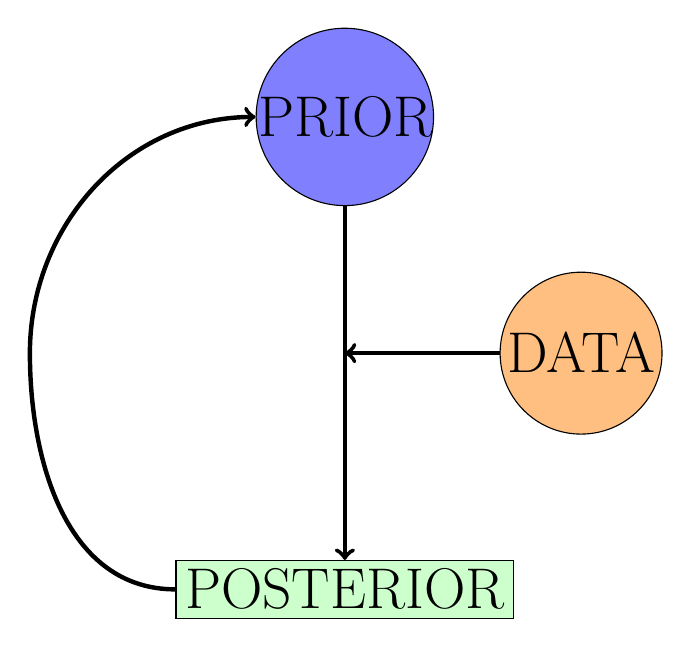
\begin{tikzpicture}
%
\node[draw,circle,fill=blue!50,inner sep=0pt,text width=2.2cm,align=center] (A) at (7,3) {\huge PRIOR};

%
\node[draw,circle,fill=orange!50,inner sep=0pt,text width=2cm,align=center] (B) at (10,0) {\huge DATA};
\node [draw,fill=green!20] (C) at (7,-3) {\huge POSTERIOR};


\draw[ultra thick,->] (A) -- (C);
\draw[ultra thick, ->]   (B) -- (7,0);
\draw [ultra thick, ->] (C.west) to [out=180, in=-90] (3, 0) to [out=90, in=-180] (A.west);

\end{tikzpicture}

\end{center}
For more details see e.g. \cite{Gelman:2014}, \cite{Hoff:2009}.
\end{frame}


%%%%%%%%%%%%%%%%%%%%%%%%%%%%%%%%%%%%%%%%%%%%%%%%%%%%%%%%%%%%%%%%%%%%%%%%
%%%%%%%%%%%%%%%%%%%%%%%%%%%%%%%%%%%%%%%%%%%%%%%%%%%%%%%%%%%%%%%%%%%%%%%%
%%%%%%%%%%%%%%%%%%%%%%%%%%%%%%%%%%%%%%%%%%%%%%%%%%%%%%%%%%%%%%%%%%%%%%%%
\begin{frame}[t]

\frametitle{Bayesian inference}

Makes fundamental distinction between
\begin{itemize}
\justifying
\item Observable quantities $\bm{y}$, i.e.~the data\vspace{2mm}
\item Unknown quantities $\bm\theta$\vspace{1mm}
\begin{itemize}
\item $\bm\theta$ can be statistical parameters, missing data, mismeasured data, $\hdots$\vspace{1mm}
\item[$\rightarrow$] parameters are treated as random variables\vspace{1mm}
\item[$\rightarrow$] in the Bayesian framework, we make probability statements about model parameters\vspace{2mm}
\end{itemize}
\item[!] in the Frequentist framework, parameters are fixed non-random quantities and the probability statements concern the data\vspace{2mm}
\end{itemize}

As with any statistical analysis, we start building a model which specifies $p(y \mid \theta)$\\ \vspace{2mm}

This is the \alert{sampling distribution}, which relates all variables into a \alert{\lq full probability model'}.
\end{frame}

%%%%%%%%%%%%%%%%%%%%%%%%%%%%%%%%%%%%%%%%%%%%%%%%%%%%%%%%%%%%%%%%%%%%%%%%
\frame{
\frametitle{Bayesian inference [continued]}
From a Bayesian point of view\vspace{1mm}
\begin{itemize}
\justifying
\item  $\bm\theta$ is unknown so should have a \alert{probability distribution} reflecting
     our uncertainty about it before seeing the data\vspace{1mm}
     \begin{itemize}
     \item[$\rightarrow$] need to specify a \alert{prior distribution} $p(\bm\theta)$\vspace{2mm}
     \end{itemize}
\item $\bm{y}$ is known so we should condition on it\vspace{1mm}
     \begin{itemize}
     \item[$\rightarrow$] use \textbf{Bayes theorem} to obtain conditional probability distribution
      for unobserved quantities of interest given the data:
      \alert{$$p(\bm\theta \mid \bm{y})= \frac{ p(\bm{y} \mid \bm\theta)\,p(\bm\theta)}
                         {p(\bm{y})}
	\propto p(\bm{y} \mid \bm\theta)\,p(\bm\theta)$$}
        \item[] This is the \alert{posterior distribution}.\vspace{2mm}
     \end{itemize}
\end{itemize}
The prior distribution $p(\bm\theta)$, expresses our uncertainty about $\bm\theta$ \alert{before} seeing the data.\vspace{2mm}

The posterior distribution $p(\bm\theta \mid \bm{y})$, expresses our uncertainty about $\bm\theta$ \alert{after} seeing the data.
}

%\begin{frame}[t]
%
%\frametitle{Components of a Bayesian analysis}
%
%In a Bayesian framework we need to explicitly state\vspace{1mm}
%\begin{itemize}
%\item a reasonable opinion concerning the plausibility
%   of different values of the the parameters (e.g. $\phi_i$)
%  {\it excluding} the evidence from the data in hand
%  (the \alert{prior distribution})\vspace{1mm}
%\item the support for different values of the parameters
%    based {\it solely} on data under study (the \alert{likelihood}),\vspace{1mm}
%\end{itemize}
%and to combine these two sources to produce\vspace{1mm}
%\begin{itemize}
%\item a final opinion about the parameters
%   (the \alert{posterior distribution})
%\end{itemize}
%
%\vspace{2mm}
%The final combination is done using Bayes theorem (and only simple rules of probability), which essentially weights the likelihood from the trial with the relative plausibilities defined by the prior distribution
%
%\vspace{2mm}
%One can view the Bayesian approach as a formalisation of the process
%of learning from experience
%\end{frame}

\begin{frame}[t]

\frametitle{Bayesian inference: the posterior distribution}

Posterior distribution forms basis for all inference --- can
be summarised to provide:\vspace{2mm}
\begin{itemize}
\justifying
\item point and interval estimates of Quantity of Interest (QOI), e.g. treatment effect, small area estimates, $\hdots$\vspace{2mm}
\item point and interval estimates of any function of the parameters\vspace{2mm}
\item probability that QOI exceeds a critical threshold\vspace{2mm}
\item prediction of QOI in a new unit\vspace{2mm}
\item prior information for future experiments, trials, surveys, $\hdots$\vspace{2mm}
\item inputs for decision making\vspace{2mm}
\item $\hdots$
\end{itemize}
\end{frame}
%%%%%%%%%%%%%%%%%%%%%%%%%%%%%%%%%%%%%%%%%%%%%%%%%%%%%%%%%%%%%%%%%%%%%%%%
%\section{Computation} 
\frame{\huge \red 
\begin{center}
\textbf{Computation}
\end{center}
}

%%%%%%%%%%%%%%%%%%%%%%%%%%%%%%%%%%%%%%%%%%%%%%%%%%%%%%%%%%%%%%%%%%%%%%%%

\begin{frame}
\frametitle{Why is computation important?}

\begin{itemize}
\justifying
\item Bayesian inference centres around the posterior distribution
   $$p(\boldsymbol{\theta} |\bm{y}) \propto p(\bm{y}|\boldsymbol{\theta}) \times p(\boldsymbol{\theta})$$
   where $\bm\theta$ is typically a large vector of parameters
   $\boldsymbol{\theta} = \left\{\theta_1, \theta_2,....,\theta_k\right\}$\\ \vspace{2mm}
\item $p(\bm{y}| \boldsymbol{\theta})$ and $p(\boldsymbol{\theta})$ will often be available in
   closed form, but $p(\boldsymbol{\theta} | \bm{y})$ is usually not analytically
   tractable, and we want to \\ \vspace{1mm}
   \begin{itemize}
   \item obtain marginal posterior $$p(\theta_i |\bm{y})= \int p(\boldsymbol{\theta} |\bm{y})\,\, d\boldsymbol{\theta}_{(-i)}$$
      where $\boldsymbol{\theta}_{(-i)}$ denotes the vector of $\theta$s excluding $\theta_i$\\ \vspace{2mm}
   \item calculate properties of $p(\theta_i |\bm{y})$, such as mean
   $(=\int \theta_i p(\theta_i|\bm{y}) d\theta_i)$, tail areas
   $(=\int_T^{\infty} p(\theta_i|\bm{y}) d\theta_i)$ etc.\vspace{2mm}
   \end{itemize}
%\item [$\rightarrow$] numerical integration becomes vital 
\end{itemize}

%\begin{itemize}
%\item Simulation based methods (e.g. MCMC)
%\item \red{Approximate methods}
%\end{itemize}
\end{frame}
%%%%%%%%%%%%%%%%%%%%%%%%%%%%%%%%%%%%%%%%%%%%%%%%%%%%%%%%%%%%%%%%%%%%%%%%
\begin{frame}
\frametitle{Approaches to computation}
\begin{itemize}
\item \alert{Simulation-based} methods 
\begin{itemize}
\justifying
\item Markov Chain Monte Carlo (MCMC): class of algorithm to sample from the posterior distribution (when not available in a closed form)
\item MCMC methods are flexible and able to deal with virtually any type of data and model, but they  involve computationally- and time- intensive simulations to obtain the posterior distribution for the parameters. For this reason the complexity of the model and the database dimension often remain fundamental issues. 
\item Software: BUGS, JAGS, STAN, \texttt{MCMCglmm, CARBayes} R packages,...
\end{itemize}
\item \alert{Approximate} methods
\begin{itemize}
\justifying
\item The Integrated Nested Laplace Approximation (INLA) algorithm proposed by \cite{Rue:2009} is a \alert{\textit{deterministic}} algorithm for Bayesian inference.
\pause\item The INLA algorithm is designed for the class of \alert{\textit{latent Gaussian models}} and compared to MCMC it provides (as) accurate results in a shorter time.
\pause\item INLA has become very popular amongst statisticians and applied researchers  and in the past few years the number of papers reporting usage and extensions of the INLA method has increased considerably (see \cite{INLAreview:2017}).
\end{itemize}
\end{itemize}
%\vspace{-2cm}
%\begin{center}
%\includegraphics[scale=0.3,angle=90]{./Figures/citations.ps}
%\end{center}
\end{frame}
%%%%%%%%%%%%%%%%%%%%%%%%%%%%%%%%%%%%%%%%%%%%%%%%%%%%%%%%%%%%%%%%%%%%%%%%
\begin{frame}
\frametitle{INLA}

\centering{\alert{\url{http://www.r-inla.org/}}}
\vspace{.2cm}

\begin{itemize}
\justifying 
\item The website contains source code, examples, papers and reports discussing the theory and applications of {INLA}.
\item There is also a discussion forum where users can post queries and requests of help.
\item Information about how to install the \texttt{R-INLA} package (which is not available from the CRAN) are provided at \url{http://www.r-inla.org/download}
\end{itemize}

%\vspace{-.2cm}
%\begin{center}
%\includegraphics[scale=0.25,angle=90]{./Figures/RINLAsite.ps}
%\end{center}

\end{frame}
%%%%%%%%%%%%%%%%%%%%%%%%%%%%%%%%%%%%%%%%%%%%%%%%%%%%%%%%%%%%%%%%%%%%%
%\section{Latent Gaussian models (LGMs)}

\frame{
\huge \red 
\begin{center}
\textbf{Latent Gaussian models (LGMs)}
\end{center}
}
%%%%%%%%%%%%%%%%%%%%%%%%%%%%%%%%%%%%%%%%%%%%%%%%%%%%%%%%%%%%%%%%%%%%%
\begin{frame}
\frametitle{Latent Gaussian models (LGMs)}
\begin{itemize}
\justifying
\item The general problem of (parametric) inference is posited by assuming a probability model for the observed data $\bm y=\left(y_1,\ldots, y_n\right)$, as a function of some relevant parameters
\[\myblue \bm{y} \mid \bm{\theta},\bm\psi \sim p(\bm{y} \mid \bm{\theta},\bm\psi) = \prod_{i=1}^n p(y_i \mid \bm{\theta},\bm\psi) \]
\pause
\item Often (in fact for a surprisingly large range of models!), we can assume that the parameters are described by a \textbf{\red Gaussian Markov Random Field} (GMRF, \cite{GMRF:2005}) \vspace{-5pt}
\begin{eqnarray*}
&& \myblue \bm\theta\mid\bm\psi \sim \mbox{Normal}(\bm 0,\bm Q^{-1}(\bm\psi)) \\
&& \myblue \theta_i \perp\!\!\!\perp \theta_j \mid \bm\theta_{-i,j}   \Longleftrightarrow Q_{ij}(\bm \psi)=0
\end{eqnarray*}\\[-5pt]
where 
\begin{itemize}
\justifying
\item The precision matrix $\bm Q$ depends on some {\red hyperparameters $\bm\psi$}.
\item The notation ``$-i,j$'' indicates all the other elements of the parameters vector, excluding elements $i$ and $j$.
\item The components of $\bm \theta$ are supposed to be \textit{conditionally independent} (given the hyperparameters) with the consequence that $\bm Q$ is a sparse precision matrix.
\end{itemize}

%\vspace{10pt}\pause
%\item This kind of models is often referred to as \textbf{\olive Latent Gaussian models}
\end{itemize}
\end{frame}
%%%%%%%%%%%%%%%%%%%%%%%%%%%%%%%%%%%%%%%%%%%%%%%%%%%%%%%%%%%%%%%%%%%%%%%%
\begin{frame}
\frametitle{LGMs as a general framework}
\begin{itemize}
\justifying
\item In general %, we can partition $\myblue \bm \psi = (\bm\psi_1,\bm\psi_2)$ and re-express a LGM as
\myblue
\begin{eqnarray*}
\bm y \mid \bm \theta,\bm\psi & \sim & \prod_i p(y_i\mid\bm \theta,\bm\psi) \hspace{88pt}\mbox{\black (``data model'')}\\
\bm\theta \mid \bm\psi & \sim & p(\bm\theta\mid\bm\psi) = \mbox{Normal}(0,\bm Q^{-1}(\bm\psi)) \hspace{20pt}\mbox{\black (``GMRF prior'')}\\
\bm\psi & \sim & p(\bm\psi) \hspace{130pt}\mbox{\black (``hyperprior'')}\\
\end{eqnarray*}
\black 
%ie $\olive\bm\psi_1$ are the \textbf{\red hyperparameters} and $\olive\bm\psi_2$ are \textbf{\blue nuisance parameters}
\pause \vspace{10pt}
\item The dimension of $\myblue \bm\theta$ can be very large (eg 10$^2$-10$^5$).
\item Conversely,  the dimension of $\myblue \bm\psi$ must be relatively small (less than 20 is recommended) to avoid an exponential increase in the computational costs of the model.
\end{itemize}
\end{frame}
%%%%%%%%%%%%%%%%%%%%%%%%%%%%%%%%%%%%%%%%%%%%%%%%%%%%%%%%%%%%%%%%%%%%%%%%
\begin{frame}
\frametitle{LGMs as a general framework}
\begin{itemize}
\justifying
\item A very general way of specifying the problem is specifying a distribution for \myblue$y_i$ \black characterized by a parameter  \myblue$\phi_i$ \black defined (ona suitable scale) as a function of a structured additive predictor   \myblue$\eta_i$ \black, such that  \myblue$g(\phi_i)=\eta_i$ \black (e.g.\ logarithm for Poisson data):
\myblue
\begin{equation*}
\eta_i = \beta_0 + \sum_{m=1}^M \beta_m x_{mi} + \sum_{l=1}^L f_l(z_{li})
\vspace{-10pt}
\end{equation*}\black
\vspace{5pt} where
\begin{itemize}
\justifying
\item $\beta_0$ is the intercept
\item $\bm \beta=\{\beta_1,\ldots,\beta_M\}$ quantify the effect of the covariates $\bm x=(\bm x_1,\ldots, \bm x_M)$ on the response
\item $\bm f=\{f_1(\cdot),\ldots,f_L(\cdot)\}$ is a set of functions defined in terms of some covariates $\bm z=(\bm z_1,\ldots, \bm z_L)$
\end{itemize}
\vspace{5pt} and then assume 
\[\red \bm\theta=\{\beta_0,\bm \beta,\bm f \} \sim \mbox{Normal}(\bm 0,\bm Q^{-1}(\bm\psi)) = \mbox{GMRF}(\bm\psi)\]
\pause
\item \textbf{NB}: This of course implies some form of Normally-distributed marginals for $\beta_0,\bm \beta$ and $\bm f$.
\end{itemize}
\end{frame}
%%%%%%%%%%%%%%%%%%%%%%%%%%%%%%%%%%%%%%%%%%%%%%%%%%%%%%%%%%%%%%%%%%%%%%%%
\begin{frame}
\frametitle{LGMs as a general framework --- examples}
Upon varying the form of the functions $\olive f_l(\cdot)$, this formulation can accommodate a wide range of models (see \cite{Martinsetal:2012} for a review)
\vspace{5pt} \pause
\begin{itemize}
\item Standard regression
\begin{itemize}
\item $\myblue f_l(\cdot) = \mbox{NULL}$
\end{itemize}
\vspace{5pt} \pause
\item Hierarchical models
\begin{itemize}
\item $\myblue f_l(\cdot) \sim \mbox{Normal}(0,\sigma^2_f)$ %\hspace{85pt} (Exchangeable)
\item[] $\myblue \sigma^2_f\mid \bm\psi \sim \mbox{some common distribution}$
\end{itemize}
\vspace{5pt} \pause
\item Spatial and spatio-temporal models 
\begin{itemize}
\item Areal data: $\myblue f_1(\cdot) \sim \mbox{CAR}$ \hspace{46pt} (Spatially structured effects)
\item[] \white areal data: $\myblue f_2(\cdot) \sim \mbox{Normal}(0,\sigma^2_{f_2})$ \hspace{10pt}\black (Unstructured residual)
\item Geostatistical data: $\myblue f(\cdot) \sim \mbox{Gaussian field}$
\item Temporal component: $\myblue f(\cdot) \sim \mbox{RW}$
\end{itemize}
\vspace{5pt} \pause
\item Spline smoothing
\begin{itemize}
\item $\myblue f_l(\cdot) \sim \mbox{AR}(\phi,\sigma^2_\varepsilon)$
\end{itemize}
\vspace{5pt} \pause
\item Survival models, logGaussian Cox Processes, etc.
\end{itemize}
\end{frame}
%%%%%%%%%%%%%%%%%%%%%%%%%%%%%%%%%%%%%%%%%%%%%%%%%%%%%%%%%%%%%%%%%%%%%%%%
\begin{frame}
\frametitle{Back to disease mapping: Smoothed estimates of $\phi_i$}
In the context of the disease mapping:

\begin{block}{Poisson-logNormal model}
\vspace{-0.5cm}
\begin{eqnarray*}
y_i & \sim & \hbox{Poisson}(\phi_i E_i) \\
\eta_i &=& \log \phi_i  =  \beta_0 + v_i
\end{eqnarray*}
where $v_i = f(z_i)$ and $z_i$ is the area ID.
\end{block}

\begin{small}
So
\begin{eqnarray*}
v_i & \sim  & \hbox{Normal}(0, \sigma_v^2)\\
\beta_0 & \sim  & \hbox{Normal}(0, 10^6)
\end{eqnarray*}

As seen in the previous slides 
\begin{itemize}
\item Parameters: $\bm\theta=\{\beta_0, \bm{v}\}$
\item Hyperpriors:  $\psi = \{\sigma_v^2\}$
\end{itemize}

Note that 
\begin{itemize}
  \item $y_i$, $E_i$: observed and expected nb of cases in area $i$ (known data)
  \item $\phi_i=\exp (\beta_0 +  v_i)$: unknown RR in area $i$ compared with expected risk based on age and sex of population (reference area)
  \item $v_i$: area-specific random effects to take into account {\color{red}overdispersion.}
%\begin{itemize}
%\item excess variation in the observed counts due to possible errors in
%numerator and denominator data
%\item latent variable which captures the effects of unknown or unmeasured
%area level covariates
%\end{itemize}
\end{itemize}
\end{small}

\end{frame}
%%%%%%%%%%%%%%%%%%%%%%%%%%%%%%%%%%%%%%%%%%%%%%%%%%%%%%%%%%%%%%%%%%%%%%%%
\begin{frame}\frametitle{Mapping smoothed vs raw estimates of $\phi_i$}

\scalebox{0.6}{\includegraphics{Figures/Lungmales_SMRHETmap.jpg}}

\begin{itemize}
\item Shrinkage towards the mean when using a hierarchical model.
\item Higher specificity, but danger of over smoothing.
\item Important to keep the same cut points.
\item Careful to not over-interpret the maps. 
\end{itemize}
\end{frame}

%%%%%%%%%%%%%%%%%%%%%%%%%%%%%%%%%%%%%%%%%%%%%%%%%%%%%%%%%%%%%%%%%%%%%%%%
%\begin{frame}
%\frametitle{MCMC and LGMs}
%\vspace{5pt}
%\begin{itemize}
%\item (Standard) MCMC methods can perform poorly when applied to (non-trivial) LGMs. This is due to several factors
%\begin{itemize}
%\item The components of the latent Gaussian field $\myblue \bm \theta$ tend to be highly correlated, thus impacting on convergence and autocorrelation
%\item Especially when the number of observations is large, $\myblue \bm\theta$ and $\myblue\bm\psi$ also tend to be highly correlated
%\item Time to run can be very long
%\end{itemize}
%\end{itemize}
%
%\begin{itemize}
%\item Blocking and overparameterisation can \textbf{alleviate}, but rarely eliminate the problem
%\end{itemize}
%
%\end{frame}
%%%%%%%%%%%%%%%%%%%%%%%%%%%%%%%%%%%%%%%%%%%%%%%%%%%%%%%%%%%%%%%%%%%%%%%%
%\section{The INLA approach}

\frame{
\huge \red 
\begin{center}
\textbf{The INLA approach}
\end{center}
}

%%%%%%%%%%%%%%%%%%%%%%%%%%%%%%%%%%%%%%%%%%%%%%%%%%%%%%%%%%%%%%%%%%%%%%%%
\frame{
\frametitle{Laplace Approximation (LA)}
\begin{itemize}
\vfill\item Approximate an integral $\int f(x)dx = \int \exp(\log(f(x))dx$ where $f(x)$ is the density function of a random variable $X$.

%\item The second ``ingredient'' is \textbf{\red Laplace approximation.}
%\pause
\vfill\item \textbf{Main idea}: Represent $\log(f(x))$ by means of a \alert{Taylor's series expansion} evaluated in the mode $x^*$ of $X$.
\vfill\item This leads to $\red f(x)\approx \mbox{Normal}(x^*, {\sigma^2}^*)$, where ${\sigma^2}^*=-1/\left.\frac{\partial^2 \log f(x)}{\partial x^2}\right|_{x=x^*}$

%\myblue 
%\begin{small}
%\begin{eqnarray*}
%\log f(x) & \approx & \log f(x^*) +(x-x^*)\left.\frac{\partial \log f(x)}{\partial x}\right|_{x=x^*}+\frac{(x-x^*)^2}{2}\left.\frac{\partial^2 \log f(x)}{\partial x^2}\right|_{x=x^*} \\
%& = & \log f(x^*) +\frac{(x-x^*)^2}{2}\left.\frac{\partial^2 \log f(x)}{\partial x^2}\right|_{x=x^*}  \qquad \black \left(\mbox{since $\left.\frac{\partial \log f(x)}{\partial x}\right|_{x=x^*}=0$}\right)
%\end{eqnarray*}
%\end{small}
%\black \pause 
%\item Setting $\myblue {\sigma^2}^*=-1/\left.\frac{\partial^2 \log f(x)}{\partial x^2}\right|_{x=x^*}$ we can re-write \vspace{-4pt}
%\[\myblue \log f(x) \approx \log f(x^*) - \frac{1}{2  {\sigma^2}^*}(x-x^*)^2 \vspace{-4pt} \]
%or equivalently \vspace{-4pt}
%\[ \myblue \int f(x)dx = \int \exp[\log f(x)]dx \approx f(x^\star) \int \exp\left[ -\frac{(x- x^*)^2}{ 2  {\sigma^2}^*}\right] dx \vspace{-5pt}\] 
%\pause
%\item Thus, under LA, $\red f(x)\approx \mbox{Normal}(x^*, {\sigma^2}^*)$.
\end{itemize}
}


%%%%%%%%%%%%%%%%%%%%%%%%%%%%%%%%%%%%%%%%%%%%%%%%%%%%%%%%%%%%%%%%%%%%%%%%


\frame{
\frametitle{Laplace approximation --- example}
As an example we consider the case of the Gamma distribution with density function
\[
\myblue f(x)=\frac{b^a}{\Gamma(a)}\exp\left(-bx\right)x^{a-1}\qquad x,a,b>0
\]

For computing the Laplace approximation we need the following quantities:
\begin{itemize}
\item $l(x)= \log f(x)=(a-1)\log x -bx +\text{constant}$
\item $\l'(x)=\frac{\partial \log f(x)}{\partial x}=\frac{a-1}{x}-b$
\item $\l''(x)=\frac{\partial^2 \log f(x)}{\partial x^2}=-\frac{a-1}{x^2}$
\end{itemize}

\pause

Then:
\begin{itemize}
\item Solving $\displaystyle l'(x) = 0$ we obtain the mode $ x^*=\frac{a-1}{b}$ (for $a>1$).
\item Evaluating $\displaystyle -\frac{1}{l''(x)}$ at the mode gives $ {\sigma^2}^*=\frac{a-1}{b^2}$
\end{itemize}

\pause
Thus, the Laplace approximation of the Gamma distribution is
\[
\myblue \text{Gamma}(a,b) \approx \text{Normal}\left(x^*=\frac{a-1}{b},{\sigma^2}^*=\frac{a-1}{b^2}\right).
\]
}


%%%%%%%%%%%%%%%%%%%%%%%%%%%%%%%%%%%%%%%%%%%%%%%%%%%%%%%%%%%%%%%%%%%%%%%%


\frame{
\frametitle{Laplace approximation --- example}

\qquad\qquad $Gamma(a=5,b=1)$\qquad \qquad\qquad\qquad $Gamma(a=10,b=5)$\\
\vspace{-1cm}
\begin{center}
\begin{tabular}{cc}
\hspace{-0.5cm}\includegraphics[scale=0.35]{Figures/Laplace1}&
\hspace{-0.5cm}\includegraphics[scale=0.35]{Figures/Laplace2}
\end{tabular}
\end{center}
\vspace{-0.5cm}

\small{Exact and approximated values of $\int_\alpha^\beta f(x) \text{d}x$ where $f(x)$ is the density function of the $\text{Gamma}(a,b)$ distribution.}
\begin{center}
\begin{tiny}
\begin{tabular}{cc|cc}
$(a,b)$ & $(\alpha,\beta)$ & Exact value & Approximated value (Laplace)\\
\hline
$(5,1)$ & $(2,6)$ &  0.6622905 & 0.6686424 \\
$(5,1)$ & $(1,10)$& 0.9670875 & 0.9126693\\
$(10,0.5)$ & $(18,22)$ & 0.2468976 & 0.2452272\\
$(10,0.5)$ & $(10,40)$ & 0.9631765& 0.9002946 \\
\hline
\end{tabular}
\end{tiny}
\end{center}
}


%%%%%%%%%%%%%%%%%%%%%%%%%%%%%%%%%%%%%%%%%%%%%%%%%%%%%%%%%%%%%%%%%%%%%%%%
\frame{
\frametitle{Integrated Nested Laplace Approximation (INLA)}
\begin{itemize}
\item In a Bayesian LGM, the required distributions are 
\begin{eqnarray*}
\myblue p(\theta_i\mid\bm{y}) \black & = & \int p(\theta_i,\boldsymbol\psi\mid \bm{y}) d\boldsymbol\psi = \int \red p(\boldsymbol\psi\mid\bm{y}) \orange p(\theta_i \mid \boldsymbol\psi,\bm{y})\black d\boldsymbol\psi \\
\myblue p(\psi_k\mid\bm{y}) \black & = & \int\red p(\boldsymbol\psi\mid\bm{y})\black d\boldsymbol\psi_{-k}
\end{eqnarray*}
\pause

\vspace{8pt}

\item Estimate (approximate)

$\displaystyle\red p(\boldsymbol\psi\mid\bm{y})  \black = \frac{p(\boldsymbol\theta,\boldsymbol\psi\mid\bm{y})}{p(\boldsymbol\theta\mid\boldsymbol\psi,\bm{y})} \approx \left. \frac{p(\boldsymbol\psi)p(\boldsymbol\theta\mid\boldsymbol\psi)p(\bm{y}\mid\boldsymbol\theta, \bm \psi)}{\tilde{p}(\boldsymbol\theta\mid\boldsymbol\psi,\bm{y})}\right |_{\boldsymbol\theta=\hat{\boldsymbol\theta}(\boldsymbol\psi)} =: \red \tilde p(\boldsymbol\psi\mid\bm{y})$ \vspace{10pt}

\pause

\begin{eqnarray*}
\orange p(\theta_i \mid \boldsymbol\psi,\bm{y}) \myblue &=& \frac{p\left(\{\theta_i,\boldsymbol\theta_{-i}\}\mid \boldsymbol\psi,\bm{y}\right)}{p(\boldsymbol\theta_{-i}\mid\theta_j,\boldsymbol\psi,\bm{y})} \approx \\
&& \left. \frac{p(\boldsymbol\psi)p(\boldsymbol\theta\mid\boldsymbol\psi)p(\bm{y}\mid\boldsymbol\theta,\bm \psi)}{\tilde{p}(\boldsymbol\theta_{-i}\mid\theta_i,\boldsymbol\psi,\bm{y})}\right|_{\bm\theta_{-i}=\hat{\bm\theta}_{-i}(\theta_i,\boldsymbol\psi)} =: \orange \tilde p(\theta_i \mid \boldsymbol\psi,\bm{y})
\end{eqnarray*}



\vspace{5pt}
where $\tilde{p}$ indicates the Laplace approximation and $\hat{\bm{\theta}}$ is the mode
%\begin{itemize}
%\item Can do various forms of LA: ``Simplified'' (based on Taylor's expansion up to 3$^\text{rd}$ order) vs ``Full'' (more precise but more computationally expensive)
%\end{itemize}
\pause \vspace{10pt}
\item Use numerical integration to obtain the marginals
\end{itemize}
}
%%%%%%%%%%%%%%%%%%%%%%%%%%%%%%%%%%%%%%%%%%%%%%%%%%%%%%%%%%%%%%%%%%%%%%%%%%%%%%%%%%%%%%%%%%%%%%%%%%%%%%%%%%%%%%%%%%%%%%%%%%%%%%%%%%%%%%%%%%%%%%%

\frame{
\frametitle{Integrated Nested Laplace Approximation (INLA)}
\vspace{5pt}
Operationally, the INLA algorithm proceeds with the following steps:
\begin{enumerate}
\justifying
\item[1.] Explore the joint posterior for the hyperparameters $\red\tilde{p}(\boldsymbol\psi\mid\bm{y})$ 
and produce a grid of  ``good'' integration points  $\olive\{\bm\psi^{(j)}\}$ associated with the bulk of the mass, together with a corresponding set of area weights $\olive\{\Delta_j\}$: 
\vspace{-.5cm}
\begin{center}
\begin{tabular}{cc}
\hspace{-.5cm}\includegraphics[scale=0.2,angle=270]{./Figures/Chapter4-hyper_grid.pdf}&\hspace{-.5cm}
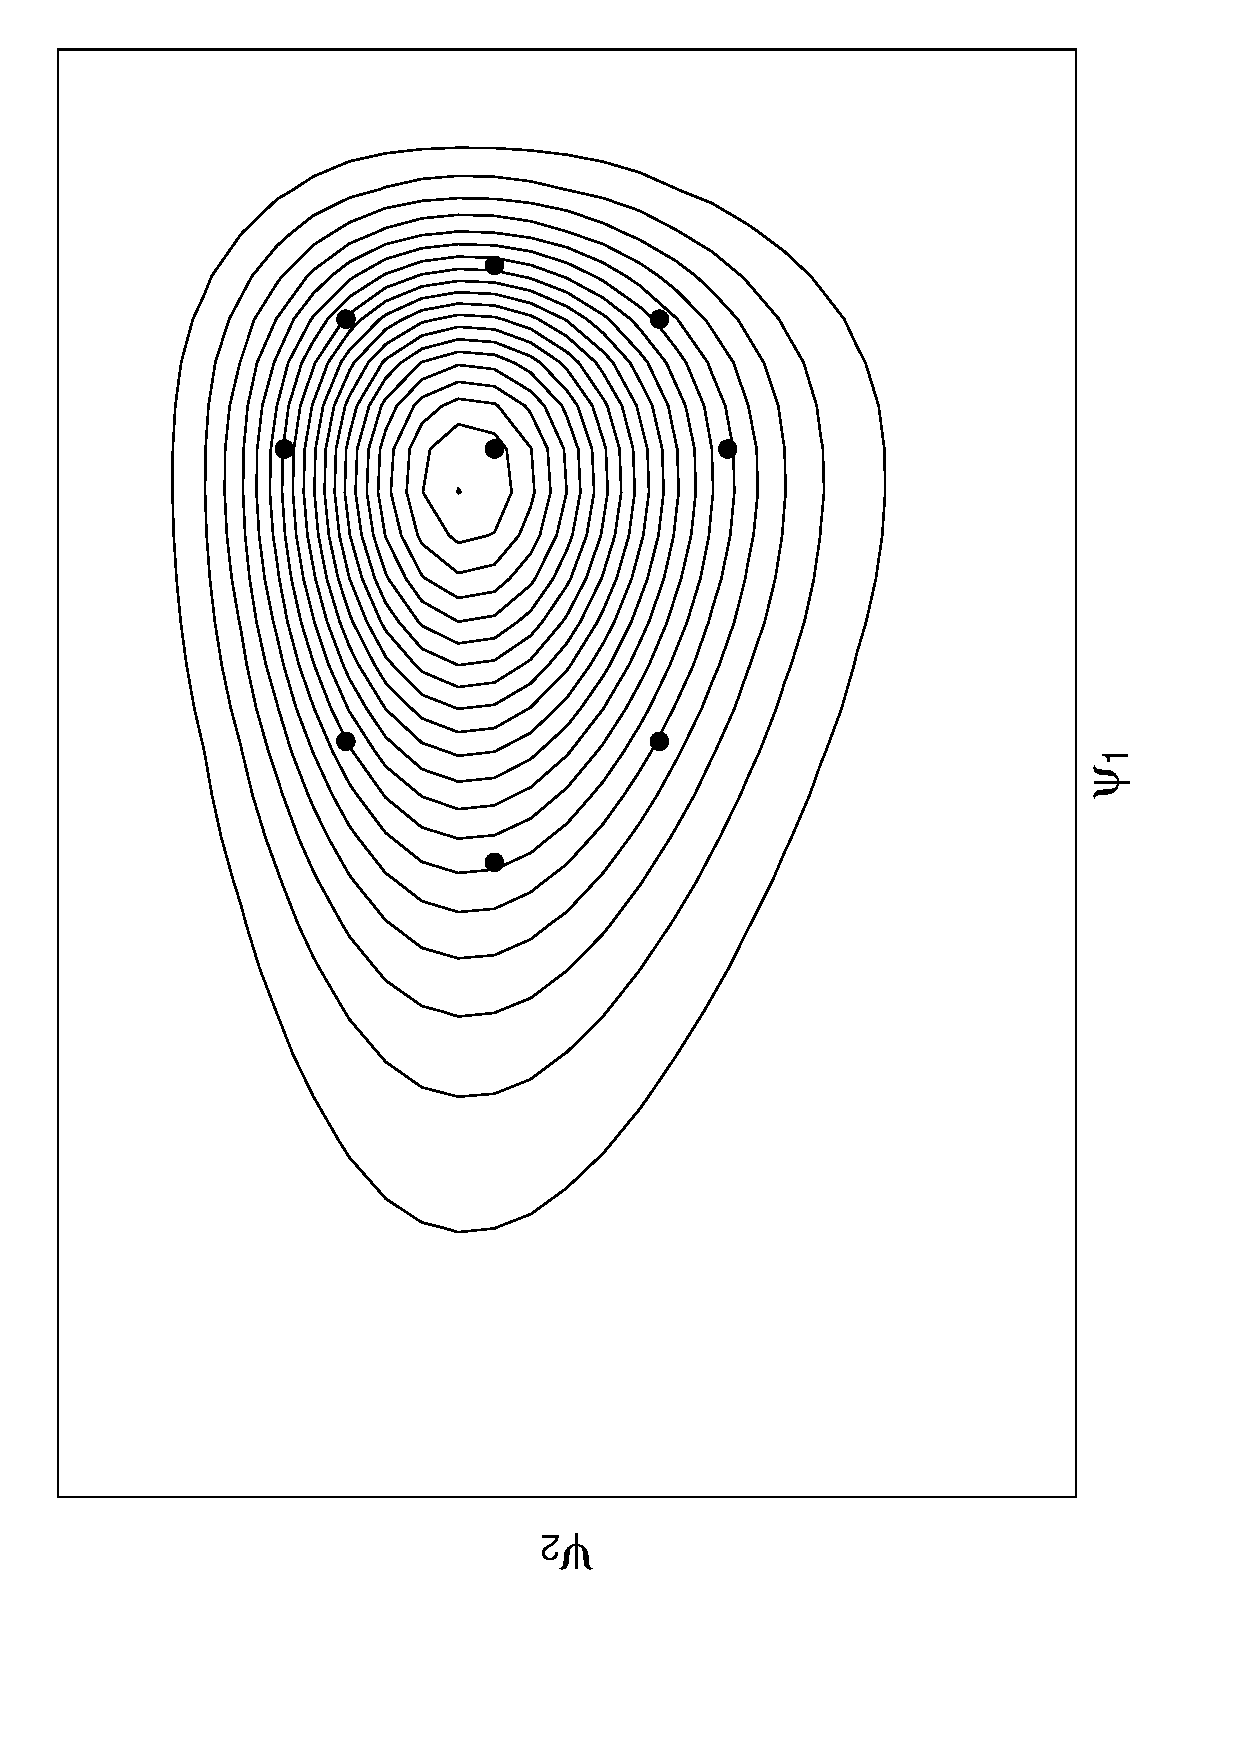
\includegraphics[scale=0.2,angle=270]{./Figures/Chapter4-hyper_CCD.pdf}\\
\small\blue{Grid strategy} & \small\blue{Central Composite Design strategy (CCD)}
\end{tabular}
\end{center}
The CCD strategy is the default one in R-INLA: it produces a lower number of points which are however enough to capture the variability of the joint distribution (see \cite{Martinsetal:2012}).

\end{enumerate}
}


%%%%%%%%%%%%%%%%%%%%%%%%%%%%%%%%%%%%%%%%%%%%%%%%%%%%%%%%%%%%%%%%%%%%%%%%

\frame{
\frametitle{Integrated Nested Laplace Approximation (INLA)}

\begin{enumerate}
\item[] Recall that the required distributions are 
\begin{eqnarray*}
\myblue p(\theta_i\mid\bm{y}) \black & \approx &  \int \red \tilde p(\boldsymbol\psi\mid\bm{y}) \orange \tilde p(\theta_i \mid \boldsymbol\psi,\bm{y})\black d\boldsymbol\psi \\
\myblue p(\psi_k\mid\bm{y}) \black & \approx & \int\red \tilde p(\boldsymbol\psi\mid\bm{y})\black d\boldsymbol\psi_{-k}
\end{eqnarray*}

\item[] After the grid exploration:
\begin{itemize}
\justifying
\vfill\item[1.] Obtain the marginal posterior $\myblue \tilde{p}(\psi_k\mid\bm{y})$ using an interpolation algorithm based on the values of the density  $\red \tilde{p}(\bm\psi\mid\bm{y})$ evaluated in the integration points $\olive\{\bm\psi^{(j)}\}$
\pause

%\vfill\item[2.] Evaluate the conditional posteriors $\orange \tilde{p}(\theta_i\mid\bm\psi^{(j)},\bm{y})$ on a grid of selected values for $\theta_i$.

\vfill\item[2.] Obtain the marginal posteriors $\myblue \tilde{p}(\theta_i\mid\bm{y})$ using \textbf{\olive numerical integration}
\begin{eqnarray*}
\myblue \tilde{p}(\theta_i\mid\bm{y}) \black \approx \sum_{j} \red \tilde{p}(\bm\psi^{(j)}\mid\bm{y})\orange \tilde{p}(\theta_i\mid\bm\psi^{(j)},\bm{y})\olive\Delta_j
\end{eqnarray*}

\end{itemize}
\end{enumerate}
}


%%%%%%%%%%%%%%%%%%%%%%%%%%%%%%%%%%%%%%%%%%%%%%%%%%%%%%%%%%%%%%%%%%%%%%%%


%\frame{
%\frametitle{Integrated Nested Laplace Approximation (INLA)}
%\textbf{Objective of Bayesian estimation}
%\begin{itemize}
%\item In a Bayesian LGM, the required distributions are 
%\begin{eqnarray*}
%\myblue p(\theta_i\mid\bm{y}) \black & = & \int p(\theta_i,\boldsymbol\psi\mid \bm{y}) d\boldsymbol\psi = \int \red p(\boldsymbol\psi\mid\bm{y}) \orange p(\theta_i \mid \boldsymbol\psi,\bm{y})\black d\boldsymbol\psi \\
%\myblue p(\psi_k\mid\bm{y}) \black & = & \int\red p(\boldsymbol\psi\mid\bm{y})\black d\boldsymbol\psi_{-k}
%\end{eqnarray*}
%\pause
%\vspace{10pt}
%\item Thus we need to estimate: 
%\begin{enumerate}
%\item[(1.)] $\red p(\boldsymbol\psi\mid\bm{y})$, from which also all the relevant marginals $\myblue p(\psi_k\mid\bm{y})$ can be obtained; \\
%{\red easy obtained through LA}\\
%\vspace{5pt}
%\pause
%\item[(2.)] $\orange p(\theta_i \mid \boldsymbol\psi,\bm{y})$, which is needed to compute the marginal posterior for the parameters
%\end{enumerate}
%\end{itemize}
%}
%%%%%%%%%%%%%%%%%%%%%%%%%%%%%%%%%%%%%%%%%%%%%%%%%%%%%%%%%%%%%%%%%%%%%%%%
%
%\frame{
%\frametitle{Integrated Nested Laplace Approximation (INLA)}
%\begin{enumerate}
%\item[1] Applying the LA we can easily obtain   
%\item[(1.)] can be easily estimated as
%\begin{eqnarray*}
%\red p(\boldsymbol\psi\mid\bm{y}) \black & = & \frac{p(\boldsymbol\theta,\boldsymbol\psi\mid\bm{y})}{p(\boldsymbol\theta\mid\boldsymbol\psi,\bm{y})} \nonumber \\ \pause
%%
%&=& \frac{p(\bm{y}\mid\boldsymbol\theta,\boldsymbol\psi)p(\boldsymbol\theta,\boldsymbol\psi)}{p(\bm{y})}\frac{1}{p(\boldsymbol\theta\mid\boldsymbol\psi,\bm{y})} \\ \pause
%%
%&=& \frac{p(\bm{y}\mid\boldsymbol\theta, \bm \psi)p(\boldsymbol\theta\mid\boldsymbol\psi)p(\boldsymbol\psi)}{p(\bm{y})}\frac{1}{p(\boldsymbol\theta\mid\boldsymbol\psi,\bm{y})} \\ \pause
%%
%& \propto & \frac{p(\boldsymbol\psi)p(\boldsymbol\theta\mid\boldsymbol\psi)p(\bm{y}\mid\boldsymbol\theta,\bm y)}{p(\boldsymbol\theta\mid\boldsymbol\psi,\bm{y})} \nonumber \\ \pause
%%
%& \approx & \left. \frac{p(\boldsymbol\psi)p(\boldsymbol\theta\mid\boldsymbol\psi)p(\bm{y}\mid\boldsymbol\theta)}{\tilde{p}(\boldsymbol\theta\mid\boldsymbol\psi,\bm{y})}\right |_{\boldsymbol\theta={\boldsymbol\theta}^*(\boldsymbol\psi)} =: \red{\tilde{p}(\boldsymbol\psi\mid\bm{y})}
%\end{eqnarray*}
%where 
%\begin{itemize}
%\item $\tilde{p}(\boldsymbol\theta\mid\boldsymbol\psi,\bm{y})$ is the Laplace approximation of $p(\boldsymbol\theta\mid\boldsymbol\psi,\bm{y})$ 
%\item $\boldsymbol\theta={\boldsymbol\theta}^*(\boldsymbol\psi)$ is its mode for a given $\bm \psi$
%\end{itemize}
%\end{enumerate}
%}
%%%%%%%%%%%%%%%%%%%%%%%%%%%%%%%%%%%%%%%%%%%%%%%%%%%%%%%%%%%%%%%%%%%%%%%%

%\frame{
%\frametitle{Integrated Nested Laplace Approximation (INLA)}
%\vspace{10pt}
%\blue{(2.)} \black is slightly more complex, because in general there will be more elements in $\boldsymbol\theta$ than there are in $\boldsymbol\psi$ and thus this computation is more expensive.
%\pause
%\vspace{10pt}
%\begin{itemize}
%\justifying
%\item \textbf{\olive Gaussian Approximation}: one easy and cheap possibility is to start from $\tilde{p}(\boldsymbol\theta\mid\boldsymbol\psi,\bm{y})$ and approximate the density of $\orange \theta_i\mid\boldsymbol\psi,\bm{y}$,  with the Gaussian marginal derived from $\tilde{p}(\boldsymbol\theta\mid\boldsymbol\psi,\bm{y})$ (using GMRF theory to derive the marginal variances). While this is very fast, the approximation is generally not very good.
%
%% i.e. using a Normal distribution, where the precision matrix is based on the Cholesky decomposition of the precision matrix $\bm{Q}$. \pause
%\vspace{10pt}
%\item \textbf{\olive Full Laplace Approximation}: alternatively, we can write $\boldsymbol\theta=\{\theta_i,\boldsymbol\theta_{-i}\}$, use the definition of conditional probability and again Laplace approximation to obtain $\orange{\tilde{p}(\theta_i\mid\boldsymbol\psi,\bm{y})}$
%%\begin{eqnarray*} 
%%\orange p(\theta_i\mid\boldsymbol\psi,\bm{y}) \black &=& \frac{p\left((\theta_i,\boldsymbol\theta_{-i})\mid \boldsymbol\psi,\bm{y}\right)}{p(\boldsymbol\theta_{-i}\mid\theta_i,\boldsymbol\psi,\bm{y})} \pause 
%%= \frac{p\left((\theta_i,\boldsymbol\theta_{-i}), \boldsymbol\psi\mid\bm{y}\right)}{p(\boldsymbol\psi\mid \bm{y})} \frac{1}{p(\boldsymbol\theta_{-i}\mid\theta_i,\boldsymbol\psi,\bm{y})} \nonumber \pause 
%%\\
%%& \propto & \frac{p\left(\boldsymbol\theta, \boldsymbol\psi\mid\bm{y}\right)}{p(\boldsymbol\theta_{-i}\mid\theta_i,\boldsymbol\psi,\bm{y})} \pause
%%\hspace{13pt} \propto \frac{p(\boldsymbol\psi)p(\boldsymbol\theta\mid\boldsymbol\psi)p(\bm{y}\mid\boldsymbol\theta,\bm \psi)}{p(\boldsymbol\theta_{-i}\mid\theta_i,\boldsymbol\psi,\bm{y})} \\ \pause
%%&\approx& \left. \frac{p(\boldsymbol\psi)p(\boldsymbol\theta\mid\boldsymbol\psi)p(\bm{y}\mid\boldsymbol\theta,\bm \psi)}{\tilde{p}(\boldsymbol\theta_{-i}\mid\theta_i,\boldsymbol\psi,\bm{y})}\right|_{\bm\theta_{-i}={\bm\theta}^*_{-i}(\theta_i,\boldsymbol\psi)} =: \orange{\tilde{p}(\theta_i\mid\boldsymbol\psi,\bm{y})}
%%\end{eqnarray*}
%\end{itemize}
%}
%%%%%%%%%%%%%%%%%%%%%%%%%%%%%%%%%%%%%%%%%%%%%%%%%%%%%%%%%%%%%%%%%%%%%%%%
%\begin{frame}[fragile]
%\frametitle{INLA in practice \hspace{0pt plus 1 filll}%\small{\texttt{http://www.statistica.it/gianluca/Talks/INLA.pdf}}
%}
%\begin{overprint}
%\begin{overlayarea}{1.1\textwidth}{1.15\textheight}
%\hspace{-.3cm}
%\begin{tikzpicture}
%\only<1-|handout:1>{
%\draw(0,0) node[align=center,rectangle,rounded corners,draw=none,font=\sffamily\fontsize{6}{7}\selectfont,text width=6.0cm](1){
%\begin{enumerate}
%\item Select a grid of points for $\psi^*_h$ and associated area weights $\Delta_h$ \& interpolate to approximate the posterior 
%\end{enumerate}
%};
%}
%
%\only<2-|handout:1>{
%\draw(6.1,0) node[align=center,rectangle,rounded corners,draw=none,font=\sffamily\fontsize{6}{7}\selectfont,text width=5.8cm](2){
%\begin{enumerate}\setcounter{enumi}{1}
%\item Weight the (conditional) marginal posteriors by the density associated with each $\psi$ on the grid
%\end{enumerate}
%};
%}
%
%\only<1-|handout:1>{
%\draw(0,-2.3) node[align=center,rectangle,rounded corners,draw=none,font=\sffamily\fontsize{6}{7}\selectfont,text width=5.8cm](3){
%\centering
%{\fontsize{4}{5}\selectfont Posterior marginal for $\psi: \myblue p(\psi \mid \bm y) \propto \frac{p(\theta,\bm y \mid \psi)p(\psi)}{p(\theta \mid \bm y, \psi)}$}\\%[-12pt] 
%\includegraphics[scale=.23, angle=90]{Figures/interp1}
%};
%}
%
%\only<2-|handout:1>{
%\draw(6.1,-2.3) node[align=center,rectangle,rounded corners,draw=none,font=\sffamily\fontsize{6}{7}\selectfont,text width=6.2cm](4){
%\centering
%{\fontsize{4}{5}\selectfont Posterior marginal for $\theta$, conditional on each $\{\psi^*_h\}$ (unweighted)}\\%[-8pt]
%\includegraphics[scale=.23]{Figures/unwgt1} 
%};
%}
%
%\only<3-|handout:1>{
%\draw(0,-4.3) node[align=center,rectangle,rounded corners,draw=none,font=\sffamily\fontsize{6}{7}\selectfont,text width=6.0cm](5){
%\begin{enumerate}\setcounter{enumi}{2}
%\item Weight the (conditional) marginal posteriors by the density associated with each $\psi$ on the grid
%\end{enumerate}
%};
%}
%
%\only<4|handout:1>{
%\draw(6.1,-4.3) node[align=center,rectangle,rounded corners,draw=none,font=\sffamily\fontsize{6}{7}\selectfont,text width=6.0cm](6){
%\begin{enumerate}\setcounter{enumi}{3}
%\item (Numerically) sum over the conditional densities to get the marginal posterior for~$\theta$ 
%\end{enumerate}
%};
%}
%
%\only<3-|handout:1>{
%\draw(0,-6.5) node[align=center,rectangle,rounded corners,draw=none,font=\sffamily\fontsize{6}{7}\selectfont,text width=6.0cm](7){
%\centering
%{\fontsize{4}{5}\selectfont Posterior marginal for $\theta$, conditional on each $\{\psi^*_h\}$ (weighted)}\\%[-12pt]
%\includegraphics[angle=90, scale=.23]{Figures/wgt1}
%};
%}
%
%\only<4|handout:1>{
%\draw(6.1,-6.5) node[align=center,rectangle,rounded corners,draw=none,font=\sffamily\fontsize{6}{7}\selectfont,text width=6.0cm](8){
%\centering
%{\fontsize{4}{5}\selectfont Posterior marginal for $\theta: \myblue p(\theta \mid \bm y)$}\\%[-5pt]
%\includegraphics[scale=.23]{Figures/marg1}
%};
%}
%\end{tikzpicture}
%\end{overlayarea}
%\end{overprint}
%\end{frame}

%%%%%%%%%%%%%%%%%%%%%%%%%%%%%%%%%%%%%%%%%%%%%%%%%%%%%%%%%%%%%%%%%%%%%%%%%%%%%


\begin{frame}
\frametitle{INLA in practice}
\[
y_i\mid\theta, \psi \sim \text{Normal}(\eta_i,\sigma^2)
\]
where $\eta_i=\theta = \mu$ and $\psi= 1/\sigma^2$. A $\text{Gamma}(a,b)$ is used as a prior  for $ \psi$.

\begin{small}
\begin{center}
\begin{tabular}{ccc}
$\red \tilde p(\psi\mid \bm y)$ & $\orange \tilde p(\theta\mid \psi^{(j)},\bm y)$ & $\tilde p(\theta\mid\bm y)=$\\
\footnotesize{$\bullet$ = grid values $\{{\psi}^{(j)}\}$}& \footnotesize{for each $\psi$ in $\{{\psi}^{(j)}\}$} & \footnotesize{$\sum_j \orange \tilde p\left(\theta\mid{\psi}^{(j)},\bm y\right)\red \tilde p\left({\psi}^{(j)}\right)\black\Delta_j$}\\
\hspace{-1cm}\includegraphics[scale=0.23]{Figures/StepBYstep1}&\hspace{-0.3cm}\includegraphics[scale=0.23]{Figures/StepBYstep2}&\hspace{-0.3cm}\includegraphics[scale=0.23]{Figures/StepBYstep3}\\

\end{tabular}
\end{center}
\end{small}
\end{frame}



%%%%%%%%%%%%%%%%%%%%%%%%%%%%%%%%%%%%%%%%%%%%%%%%%%%%%%%%%%%%%%%%%%%%%%%%%%%%%
%
%\frame{
%\frametitle{Different approximations}
%\begin{itemize}
%\justifying
%\vfill\item Because $\left(\boldsymbol\theta_{-i}\mid\theta_i,\boldsymbol\psi,\bm{y}\right)$ are reasonably Normal, the approximation works generally well.
%\item However, this strategy can be computationally expensive as $\tilde{p}(\theta_{-i}\mid\theta_i,\boldsymbol\psi,\bm{y})$ must be recomputed for each value of $\bm \theta$ and $\bm \psi$.
%\pause
%\vspace{10pt}
%\vfill\item The most efficient algorithm is the \textbf{\olive Simplified Laplace Approximation}:
%\begin{itemize}
%\vfill\item Based on a Taylor's series expansion of the Laplace approximation $\orange\tilde{p}(\theta_i\mid\boldsymbol\psi,\bm{y})$\black.
%\vfill\item This is usually corrected by including a mixing term (e.g. spline) to increase the fit to the required distribution.
%\vfill\item The accuracy of this approximation is sufficient in many applied cases and that the computing time is considerably shorter, it is the standard option.
%\end{itemize}
%\pause
%\vspace{10pt}
%\item This is the algorithm implemented by default by \texttt{R-INLA}, but this choice can be modified.
%\begin{itemize}
%\item If extra precision is required, it is possible to run the full Laplace approximation --- of course at the expense of running time!
%\end{itemize}
%\end{itemize}
%}

%%%%%%%%%%%%%%%%%%%%%%%%%%%%%%%%%%%%%%%%%%%%%%%%%%%%%%%%%%%%%%%%%%%%%%%%

%\frame{
%\frametitle{Integrated Nested Laplace Approximation (INLA)}
%So, it's all in the name... \\[10pt] 
%
%\textbf<4>{\color<4>{myblue}Integrated} \textbf<3>{\color<3>{myblue}Nested} \textbf<2>{\color<2>{myblue}Laplace Approximation}
%\begin{itemize}
% \colorize<2> \item Because Laplace approximation is the basis to estimate the unknown distributions
% \colorize<3> \item Because the Laplace approximations are nested within one another
%\begin{itemize}
%\colorize<3> \item  Since the distribution of the hyperparameters $\boldsymbol\psi$ is needed to estimate the distribution of the parameters $\boldsymbol\theta$
%%\colorize<3> \item NB: Consequently the estimation of (1.) might not be good enough, but it can be refined (eg using a finer grid)
%\end{itemize}
%\colorize<4> \item Because the required marginal posterior distributions are obtained by (numerical) integration.
%\end{itemize}
%}

\frame{
\frametitle{Summary so far}
\begin{itemize}
\justifying
\item The INLA approach is not a rival/competitor/replacement to/of MCMC, just a better option for the class of LGMs.
\medskip

\item The basic idea behind the INLA procedure is simple:


\begin{itemize}
\justifying
\item Repeatedly use Laplace approximation and take advantage of computational simplifications due to the structure of the model;
\item Use numerical integration to compute the required posterior marginal distributions.
%\item (If necessary) refine the estimation (eg using a finer grid)
\end{itemize}
\medskip
\item Complications are mostly computational and occur when:
\begin{itemize}
\justifying
\item Extending to a large number of hyperparameters;
\item Markedly non-Gaussian observations. \nocite{Blangiardo:2015}
\end{itemize}
\end{itemize}
}
%%%%%%%%%%%%%%%%%%%%%%%%%%%%%%%%%%%%%%%%%%%%%%%%%%%%%%%%%%%%%%%%%%%%%%%%
%\section{Adding a spatial structure}
\frame{
\huge \red 
\begin{center}
\textbf{Adding a spatial structure}
\end{center}
}


\frame{
\frametitle {Why adding a spatial structure?}
\begin{itemize}
\justifying
\vfill \item Poisson-logNormal model based on the assumption that
   the observations in the data set are identically distributed
   and independent.\\
 $\Rightarrow$  Independence makes much of the mathematics tractable.
\vfill \item However, data that occur close together in space (or time)
   are likely to be  correlated. \\
   $\Rightarrow$ Dependence between observations is a more
   realistic assumption.
\vfill \item Ignoring this dependence can lead to biased and inefficient inference.\\
$\Rightarrow$ {\color{red} Smooth in space} prior distribution for the random effects should allow for spatial correlation.
\end{itemize}
}
%%%%%%%%%%%%%%%%%%%%%%%%%%%%%%%%%%%%%%%%%%%%%%%%%%%%%%%%%%%%%%%%%%%%%%%%
\begin{frame}
\frametitle{A conditional spatial model}
\begin{itemize}
\item Specify the distribution of each random effect as if we knew the values of the spatial random effects in {\color{red} neighbouring areas}.
\vfill
\item We have a conditional specification since we are conditioning on knowing the neighbours.
\vfill
\item Rule for determining the neighbours of each area: most common based on common boundary.
\vfill
\item Use of conditional autoregressive distributions.
\vfill
\end{itemize}
\end{frame}
%%%%%%%%%%%%%%%%%%%%%%%%%%%%%%%%%%%%%%%%%%%%%%%%%%%%%%%%%%%%%%%%%%%%%%%%
\begin{frame}
\frametitle{Intrinsic CAR model}
\begin{block}{Common definition \cite{besag:1974}}
$$ \mathbf{u} \sim \hbox{ICAR}(\mathbf{W},\sigma^2_u)$$

Let $\partial_i =$ set of areas adjacent to $i$, $w_{ij}$  = 1 for $j \in \partial_i$, 0 otherwise
\begin{eqnarray*}
u_i \mid u_{j \;\; j\ne i} \sim \hbox{Normal}(\frac{\sum_{j \in \partial_i} u_j}{n_i}, \frac{\sigma^2_u}{n_i})
\end{eqnarray*}
\end{block}

\begin{itemize}
\item $u_i$ is smoothed towards mean risk in a set of neighbouring areas
\vfill\item Conditional variance inversely proportional to the number of neighbours (so more neighbours, less variability)
\end{itemize}
\end{frame}
%%%%%%%%%%%%%%%%%%%%%%%%%%%%%%%%%%%%%%%%%%%%%%%%%%%%%%%%%%%%%%%%%%%%%%%%

\frame{\frametitle{Poisson model with BYM random effects I}
\begin{itemize}
\vfill \item Besag, York and Mollie (BYM, \cite{Besag:1991}) recommend combining the ICAR prior and the standard normal prior to allow for both
\vfill
    \begin{itemize}
    \item spatially unstructured latent covariates $\mathbf{v}$ modelled as iid
    \item[$\Rightarrow$] global smoothing
    \item spatially correlated latent covariates $\mathbf{u}$ modelled as ICAR
    \item[$\Rightarrow$] local smoothing
    \end{itemize}
\end{itemize}
\vfill
\begin{block}{Convolution or BYM model}
\begin{eqnarray*}
y_i & \sim & \hbox{Poisson}(\phi_i E_i) \\
\log \phi_i & = & \beta_0 + v_i + u_i \\
v_i &\sim & \hbox{Normal}(0, \sigma^2_v) \\
\bf{u} & \sim & \hbox{ICAR}(\mathbf{W}, \sigma^2_u)
\end{eqnarray*}

{\small
Priors (vague, non informative): $\sigma_v^2, \sigma_u^2, \beta_0$
}
\end{block}

}
%%%%%%%%%%%%%%%%%%%%%%%%%%%%%%%%%%%%%%%%%%%%%%%%%%%%%%%%%%%%%%%%%%%%%%%%

\begin{frame}[fragile]
\frametitle{Poisson model with BYM random effects II}
\begin{itemize}

  \item Choice of the adjacency matrix (neighbours) $\rightarrow$ 2 areas are adjacent if common borders  
 \vfill  
  \item $\hbox{RR}_i = \exp(\beta_0 + v_i + u_i)$: RR in area $i$ relative to the age/sex structure (used to estimate the $E_i$)
 \vfill
  \item $\hbox{residual RR}_i = \exp(v_i + u_i)$: residual RR in area $i$ relative to the region average after adjusting for the overall risk
  
\end{itemize}
\end{frame}
%%%%%%%%%%%%%%%%%%%%%%%%%%%%%%%%%%%%%%%%%%%%%%%%%%%%%%%%%%%%%%%%%%%%%%%%
\begin{frame}
\frametitle{Neighbourhood definition}
\begin{itemize}
\vfill\item Common approach: 2 areas are neighbours if they share a common border (or point)
\vfill\item[$\rightarrow$] Adjacency matrix implemented in INLA
\vfill\item An area cannot be specified as its own neighbour
\vfill\item Adjacency matrix must be symmetric
\end{itemize}

\begin{tabular}{cc}
\includegraphics[scale=0.25,angle=0]{./Figures/nblondon} 
&\hspace{-2cm}\includegraphics[scale=0.25,angle=0]{./Figures/neighbors}
\end{tabular}

\end{frame}
%%%%%%%%%%%%%%%%%%%%%%%%%%%%%%%%%%%%%%%%%%%%%%%%%
\frame{
\frametitle{Lung cancer incidence in males, 1985-2009, England and Wales}

Here we replace the unstructured Normal random effects prior for the log relative risks by a convolution (CAR + unstructured Normal) prior:
\begin{eqnarray*}
y_i & \sim & \hbox{Poisson}(\phi_i E_i) \\
\log \phi_i & = & \beta_0 + v_i +u_i \\
v_i &\sim & \hbox{Normal}(0, \sigma^2_v) \\
\bf{u} & \sim & \hbox{ICAR}(W, \sigma^2_u)
\end{eqnarray*}
\vfill 

\begin{itemize}
\item Data: \uncover<2->{$\bm{y}$ and $\bm{E}$, observed and expected cases, $W$ adjacency matrix} 
\item Priors: \uncover<3->{$\sigma^2_v$, $\sigma^2_u$, $\beta_0$}

\item Parameters of interest: 
\uncover<4->{
\begin{itemize}
\item residual RR $\hbox{resRR}=\exp(v_i + u_i)$
\end{itemize}
}
\end{itemize}
}
%%%%%%%%%%%%%%%%%%%%%%%%%%%%%%%%%%%%%%%%%%%%%%%%%
%%%%%%%%%%%%%%%%%%%%%%%%%%%%%%%%%%%%%%%%%%%%%%%%%%%%%%%%%%%%%%%%%%%%%%%%
\frame{\frametitle{Residual RR of lung cancer incidence in males, 1985-2009, England and Wales II}
\noindent \begin{minipage}[t]{3.5cm}
{\footnotesize
\begin{itemize}
\item[SMR] non smoothed RR
\item[HET] non spatially smoothed residual RR $\exp(v)$
\item[ICAR] spatially smoothed residual RR $\exp(u)$
\item[BYM] spatially and non spatially smoothed residual RR $\exp(v+u)$
\end{itemize}}
\end{minipage}\hfill
\noindent \begin{minipage}[t]{7cm}
\begin{center}
{\scalebox{0.5}{
\includegraphics{Figures/Lungmales_4maps.jpg}
}}
\end{center}
\end{minipage}
}
%%%%%%%%%%%%%%%%%%%%%%%%%%%%%%%%%%%%%%%%%%%%%%%%%%%%%%%%%%%%%%%%%%%%%%%%

\frame{\frametitle{Other conditional autoregressive structures}
\begin{itemize}
\vfill \item BYM is not the only option to account for spatial correlation at small area.
\vfill \item A popular alternative consists in the modelling proposed by Leroux (\cite{leroux2000estimation}). 
\end{itemize}
\vfill

\begin{block}{Leroux model}
\begin{eqnarray*}
u_i \mid u_{j \;\; j\ne i} \sim \hbox{Normal}(\frac{\rho\sum_{j \in \partial_i} u_j + (1-\rho)\mu}{n_i\rho+1-\rho}, \frac{\sigma^2_u}{n_i\rho+1-\rho})
\end{eqnarray*}\end{block}

\begin{itemize}
\item The additional parameter $\rho$ governs the amount of spatial autocorrelation.
\item As $\mu$ is included in the formulation there is no need for an intercept in the log-linear specification, i.e. $\log \phi_i  =  u_i $.
\item Priors: $\sigma_u^2$, $\mu$, $\rho$  
\item Not directly available in INLA .
\end{itemize}
}
%%%%%%%%%%%%%%%%%%%%%%%%%%%%%%%%%%%%%%%%%%%%%%%%%%%%%%%%%%%%%%%%%%%%%%%%
\begin{frame}
\frametitle{Posterior Probability}
\begin{itemize}
\vfill \item Mapping the posterior mean relative risk does not make full use of the output of the Bayesian analysis that provides, for each area, samples from the whole posterior distribution of the relative risk.
\vfill \item Mapping the probability that a relative risk is greater than a specified threshold of interest has been proposed by several authors (e.g. \cite{Clayton1992}).
\vfill \item Very effective method to identify areas characterised by elevated risk.
\end{itemize}
\end{frame}
%%%%%%%%%%%%%%%%%%%%%%%%%%%%%%%%%%%%%%%%%%%%%%%%%%%%%%%%%%%%%%%%%%%%%%%%

\frame{ \frametitle{How to classify areas as having elevated risk}
\begin{itemize}
\vfill \item We define the decision rule $D(c, RR_0)$, which depends
    \begin{itemize}
        \vfill \item $\rightarrow$ on a cutoff probability $c$\\[5pt]
        \vfill \item $\rightarrow$ a reference threshold $RR_0$.\\[5pt]
    \end{itemize}
\vfill \item Area $i$ is classified as having an elevated risk according to
{\centering $D(c, RR_0) \leftrightarrow \hbox{Prob}(RR_i > RR_0) > c$}.

\pause\vfill \item \cite{richardson2004interpreting} presented a simulation study to find the best parameters $c$ and $RR_0$ and proposed $c=0.8$ and $RR_0=1$.

 \item Posterior probabilities of interest
\begin{itemize}
  \item $\hbox{Prob}(RR_i > 1) = \hbox{Prob}(e^{\beta_0 + v_i + u_i} > 1)$
  \item $\hbox{Prob}(e^{v_i + u_i} > 1) = \hbox{Prob}(e^{(\beta_0 +v_i + u_i} > e^{\alpha}) = \hbox{Prob}(RR_i > e^{\beta_0})$.
\end{itemize}
\end{itemize}
}
%%%%%%%%%%%%%%%%%%%%%%%%%%%%%%%%%%%%%%%%%%%%%%%%%%%%%%%%%%%%%%%%%%%%%%%%

\begin{frame}
    \frametitle{Lung cancer incidence in males, 1985-2009, England and Wales}
    \vspace{-0.5cm}
\begin{center}
\scalebox{0.2}{\includegraphics{Figures/Lungmales_BYMproba.jpg}}

Map of the smoothed residual RRs and posterior probabilities that the RR is above the average risk
\end{center}
\end{frame}
%%%%%%%%%%%%%%%%%%%%%%%%%%%%%%%%%%%%%%%%%%%%%%%%%%%%%%%%%%%%%%%%%%%%%%%%
\begin{frame}
    \frametitle{Lung cancer incidence in males, 1985-2009, England and Wales}
    \vspace{-0.5cm}
\begin{center}
\scalebox{0.17}{\includegraphics{Figures/Lungmales_rankedBYM.jpg}}
\end{center}
\end{frame}
%%%%%%%%%%%%%%%%%%%%%%%%%%%%%%%%%%%%%%%%%%%%%%%%%%%%%%%%%%%%%%%%%%%%%%%%
\frame{
\huge \red 
\begin{center}
\textbf{From space to space-time}
\end{center}
}
%%%%%%%%%%%%%%%%%%%%%%%%%%%%%%%%%%%%%%%%%%%%%%%%%%%%%%%%%%%%%%%%%%%%%%%%
\frame{\frametitle{Disease mapping: Extending space to space-time}
\begin{itemize}
\vfill \item Disease mapping is usually carried out on aggregated
data over a time period.
\vfill \item Rather than suppressing the time
dimension, it can be interesting to use models that combine the
space and time dimension.
\vfill \item The stability (or not) of the
spatial pattern can aid interpretation.
\vfill \item The specific
space-time components of the model can potentially pinpoint
unusual/emerging hazards.
\vfill \item Data $\hbox{y}_{it}$ and
$\hbox{E}_{it}$: the observed and expected number of cases in area $i$ at time $t$\\
$E_{it} = \sum_k n_{itk} r_k$, where $r_k$ reference rate for stratum (age, gender,...)
\end{itemize}
}
%%%%%%%%%%%%%%%%%%%%%%%%%%%%%%%%%%%%%%%%%%%%%%%%%%%%%%%%%%%%%%%%%%%%%%%%

\frame{\frametitle{Schematic representation I}
\begin{center}
\scalebox{0.5}
{\includegraphics{Figures/representation_ST1.jpg} }
\end{center}
}

\frame{\frametitle{Schematic representation II}
\begin{center}
\scalebox{0.5}
{\includegraphics{Figures/representation_ST.jpg} }
\end{center}
}

%%%%%%%%%%%%%%%%%%%%%%%%%%%%%%%%%%%%%%%%%%%%%%%%%%%%%%%%%%%%%%%%%%%%%%%%
\begin{frame}\frametitle{Georgia low birth weight - temporal SMRs}
\begin{tabular}{cc}
\begin{minipage}[c][4cm]{0.5\textwidth}
\begin{center}
\scalebox{0.45}
{\includegraphics{Figures/SMRSPatialGeorgia}}
\end{center}
\end{minipage}

&

\hspace{1cm}\begin{minipage}[c][5cm]{0.4\textwidth}
\begin{itemize}
\vfill\item Low birth weight babies ($<2500$g) born between 2000 and 2010 in Georgia (county level).
\vfill\item County specific yearly SMR
\end{itemize}
\end{minipage}
\end{tabular}
\end{frame}
%%%%%%%%%%%%%%%%%%%%%%%%%%%%
%\begin{frame}
%\frametitle{Ohio Lung cancer - temporal SMRs }
%
%\begin{itemize}
%\item Lung cancer deaths in Ohio for 1968-1988
%\end{itemize}
%
%\begin{minipage}{0.4\linewidth}
%\begin{center}
%\scalebox{0.22}
%{\includegraphics{Figures/ohio_smr_year_72.jpeg}}
%\end{center}
%\end{minipage}
%\hfill
%\begin{minipage}{0.4\linewidth}
%\begin{center}
%\scalebox{0.22}
%{\includegraphics{Figures/ohio_smr_year_76.jpeg}}
%\end{center}
%\end{minipage}
%\vfill
%\begin{minipage}{0.4\linewidth}
%\begin{center}
%\scalebox{0.22}
%{\includegraphics{Figures/ohio_smr_year_84.jpeg}}
%\end{center}
%\end{minipage}
%\hfill
%\begin{minipage}{0.4\linewidth}
%\begin{center}
%\scalebox{0.22}
%{\includegraphics{Figures/ohio_smr_year_88.jpeg}}
%\end{center}
%\end{minipage}
%\end{frame}
%%%%%%%%%%%%%%%%%%%%%%%%%%%%%%%%%%%%%%%%%%%%%%%%%%%%%%%%%%%%%%%%%%%%%%%
\begin{frame}
\frametitle{Georgia low birth weight - temporal SMRs for selected counties}
\begin{center}
Log SMR time trends in 6 counties of Georgia
\scalebox{0.35}
{\includegraphics{Figures/SMRTrendGeorgia}}\\
``Messy'' trends - different variability for different areas
\end{center}
\end{frame}
%%%%%%%%%%%%%%%%%%%%%%%%%%%%%%%%%%%%%%%%%%%%%%%%%%%%%%%%%%%%%%%%%%%%%%%

\begin{frame}[fragile]
\frametitle{Spatio-temporal model}

\begin{eqnarray*}
\hbox{y}_{it} & \sim & \hbox{Poisson}(\phi_{it}\hbox{E}_{it}) \\
\log\phi_{it} & = & \beta_0 + u_i + v_i + ?\\
\end{eqnarray*}
where
\begin{itemize}
\item $\beta_0$ overall log RR in Georgia over the 21-year period;
\item $v_i \sim \hbox{Normal}(0, \sigma^2_v)$ spatially unstructured RE;
\item $\mathbf{u} \sim \hbox{ICAR}(\mathbf{W}, \sigma^2_u)$ spatially structured RE.
\end{itemize}

\vfill\pause\begin{block}{How do we model time?}
Contrary to spatial models, there is a natural
order to any time series data which is used in specifying the
models.
\end{block}
\end{frame}
%%%%%%%%%%%%%%%%%%%%%%%%%%%%%%%%%%%%%%%%%%%%%%%%%%%%%%%%%%%%%%%%%%%%%%%

\frame{ \frametitle{Autoregressive models}

\begin{itemize}

\vfill\item \textbf{Idea}: predict an output based on the previous outputs.

\vfill\item Let $ {\bm \lambda}  = (\lambda_1, \ldots, \lambda_T)$ be a
time ordered sequence of parameters

\vfill\item An autoregressive Gaussian model for $\bm\lambda$ is defined by:
    \begin{itemize}
    \item a time lag $p$
    \item a set of coefficients $\{b_1, \ldots b_p\}$
    \end{itemize}
so that
$$\lambda_t = b_1\lambda_{t-1} + b_2\lambda_{t-2}+ \ldots +b_p\lambda_{t-p}+ \epsilon_t, \quad \epsilon_t \sim \hbox{N}(0,\sigma^2_{\epsilon})$$

equivalently
\vspace{-0.1cm}$$\lambda_t |\lambda_{t-1}, \lambda_{t-2}, \ldots
\lambda_{t-p} \sim N\left(\sum_{j=1}^{p} b_j \lambda_{t-j},
\sigma^2_{\epsilon}\right), \quad t= p+1, \ldots, T$$
\end{itemize}
}

\begin{frame}
\frametitle{Random walk of order 1, RW(1)}
%$$\theta_t = \theta_{t-1} + \epsilon_t, \quad \epsilon_t \sim \hbox{N}(0,\sigma^2_{\epsilon}) $$
\vspace{-0.4cm}

%    \item  This process is non stationary (variance doesn't exist)
\begin{eqnarray*}
        \lambda_t & = & \lambda_{t-1} + \epsilon_t, \quad \lambda_{t-1}  = \lambda_{t-2} + \epsilon_{t-1}\\
        \Rightarrow \lambda_t & = & \lambda_{t-2} + \epsilon_{t-1} + \epsilon_t\\
        \Rightarrow \lambda_t & = & \lambda_{0} + \epsilon_{1}+ \ldots + \epsilon_t\\
        \text{Mean  } \hbox{E}(\lambda_t)  &=& \lambda_0\\
        \text{Variance  } \hbox{Var}(\lambda_t) &=& \hbox{Var}(\epsilon_{1}) + \ldots + \hbox{Var}(\epsilon_t)=t\sigma_\epsilon^2 \rightarrow \infty \text{ if } t\rightarrow \infty
        \end{eqnarray*}
\begin{itemize}        
  \vfill  \item It only models the \textcolor{red}{difference of levels on consecutive time points} ($\lambda_t-\lambda_{t-1}=\epsilon_{t}$)
    \end{itemize}
\vspace{0.5cm}    
%{\footnotesize stationary process if mean and variance independent of time $t$}
\end{frame}

\begin{frame}
    \frametitle{Random walk of order 1, RW(1)}
 \begin{center}
\scalebox{0.5}{\includegraphics{Figures/RW1new.jpeg} }
\end{center}
\end{frame}

\begin{frame}
\frametitle{Random walk of order 2, RW(2)}
$$\lambda_t = 2\lambda_{t-1} - \lambda_{t-2} + \epsilon_t$$

\begin{itemize}
%    \vfill\item  This process is non stationary
    
\item It only models a \textcolor{red}{linear combination of levels on consecutive time points} ($\lambda_t-2\lambda_{t-1}+\lambda_{t-2}=\epsilon_{t}$)
    \end{itemize}
%\end{frame}

%\begin{frame}
%    \frametitle{Comparison between RW(1) and RW(2)}
\begin{tabular}{cc}
\begin{minipage}[c]{0.5\textwidth}
\begin{center}
\scalebox{0.3}{\includegraphics[trim=0.7cm 0cm 0cm 0cm,clip]{Figures/ex_RW.jpeg} }\\
\vspace{-0.3cm}
\end{center}
\end{minipage}
&
\begin{minipage}[c]{0.4\textwidth}
\begin{itemize}
\item Simulated data from a sine curve, then  RW(1) and RW(2) models fitted\\
\item RW(2) model provides greater smoothing than the RW(1) model (dots=observed data)
\end{itemize}
\end{minipage}
\end{tabular}
\end{frame}

\frame{ \frametitle{Conditional distributions for a RW(1) and RW(2)}

\begin{itemize}
\vfill \item The conditional distributions $p(\lambda_t |\bm \lambda_{-t})$, where
$\bm \lambda_{-t}$ represent the  vector of $\lambda$s with
$\lambda_t$ removed, can be derived.
\item \textbf{RW1}: The conditional distribution of $\lambda_t$ involves
$\lambda_{t-1}$:
\begin{eqnarray*}
p(\lambda_t |\bm \lambda_{-t},\sigma^2_{\epsilon})=
N(\lambda_{t-1},\sigma^2_{\epsilon})
\end{eqnarray*}
\vfill \item \textbf{RW2}: The conditional distribution of $\lambda_t$ involves
$\lambda_{t-2}, \lambda_{t-1}$:    
\begin{eqnarray*}
p(\lambda_t |
    \bm\lambda_{-t},\sigma^2_{\epsilon})=
       N(2\lambda_{t-1}-\lambda_{t-2} ,\sigma^2_{\epsilon})
\end{eqnarray*}
%\vfill \item Similar form with the spatial
%autoregression case (ICAR) 
%{\footnotesize $$\hbox{Recall: } p(X_i | X_{-i}) = \hbox{Normal}\left(\frac{\sum_{j} w_{ij} X_j}{\sum_{j} w_{ij}}, \frac{\sigma^2_u}{\sum_{j}  w_{ij}}\right)$$}
%    \begin{itemize}
%    \vfill \item time neighbours of $t$ are $t-1$ and $t+1$
%    \vfill \item if $t=1$ or $t=T$, only 1 neighbour: $t_2$ and $t_{T-1}$
%    \vfill \item weights: 1
%    \end{itemize}
\end{itemize}
}
%%%%%%%%%%%%%%%%%%%%%%%%%%%%%%%%%%%%%%%%%%
\begin{frame}
\frametitle{Back to disease mapping: Simple additive space-time structure}
%\begin{block}{Model 4}
\begin{eqnarray*}
\hbox{y}_{it} & \sim & \hbox{Poisson}(\phi_{it}\hbox{E}_{it}) \\
\log\rho_{it} & = & \beta_0 + u_i + v_i + \alert{\lambda_t} + \alert{\gamma_t}\\
\end{eqnarray*}
%\end{block}
where
\begin{itemize}
\item $\beta_0$ overall log RR in Georgia over the 11-year period
\item $v_i \sim \hbox{Normal}(0, \sigma^2_v)$ spatially unstructured RE
\item $\mathbf{u} \sim \hbox{ICAR}(\mathbf{W}, \sigma^2_u)$ spatially structured RE
\item \alert{$\lambda_t  \sim \hbox{RW}(1)$ temporally structured RE with variance parameter $\sigma^2_{\lambda}$}
\item \alert{$\gamma_t  \sim \hbox{Normal}(0, \sigma^2_{\gamma})$ temporally unstructured RE}
\end{itemize}
\end{frame}
%%%%%%%%%%%%%%%%%%%%%%%%%%%%%%%%%%%%%%%%%%
\begin{frame}
\frametitle{Adding a space-time interaction}
\begin{itemize}
\item The model can be extended by including {\bf space-time interactions parameters}, $\delta_{it}$.
\item The interactions can be modelled in different ways depending on which parameters are supposed to interact
\end{itemize}
\begin{eqnarray*}
\hbox{y}_{it} & \sim & \hbox{Poisson}(\phi_{it}\hbox{E}_{it}) \\
\log \phi_{it} & = & \beta_0 + v_i + u_i  + \lambda_t  + \gamma_t + \color{blue}{\delta_{it}}\\
v_i + u_i & = & \; \hbox{(BYM = HET + ICAR)}\\
\lambda_t & \sim & \hbox{RW(1)}\\
\gamma_t & \sim & N(0,\sigma^2_{\gamma})
\end{eqnarray*}

\begin{enumerate}[label=(\roman*)]
\item $v_i$ and $\gamma_t$ interact: non structured; 
\item $v_i$ and $\lambda_t$ interact: dependence in time but independent for each area;
\item $u_i$ and $\gamma_t$ interact: dependence in space but independent for each time point;
\item $u_i$ and $\lambda_t$ interact: completely structured. 
\end{enumerate}

%\begin{footnotesize}
%\begin{center}\begin{tabular}{lcl}
%\hline
%Interaction & Parameter interacting & Matrix Rank \\
%\hline
%I & $v_i$ and $\lambda_t$ & $nT$\\
%II &  $v_i$ and $\gamma_t$ & $n(T-1)$ for RW1\\
% & & $n(T-2)$ for RW2\\
%III & $\lambda_t$ and $u_i$ & $(n-1)T$\\
%IV & $u_i$ and $\gamma_t$ & $(n-1)(T-1)$ for RW1\\
%& &  $(n-1)(T-2)$ for RW2\\
%\hline
%\end{tabular}\end{center}
%\end{footnotesize}
\end{frame}
%%%%%%%%%%%%%%%%%%%%%%%%%%%%%%%%%%%%%%%%%%
\begin{frame}\frametitle{Georgia low birth weight - results with space-time interaction}
\begin{itemize}
\item Assuming a type I interaction (non structured)
\end{itemize}
\begin{eqnarray*}
\hbox{y}_{it} & \sim & \hbox{Poisson}(\phi_{it}\hbox{E}_{it}) \\
\log \phi_{it} & = & \beta_0 + v_i + u_i  + \lambda_t  + \gamma_t + \color{blue}{\delta_{it}}\\
...\\
\delta_{it} &\sim& N(0,\sigma^2_{\delta})
\end{eqnarray*}

\vspace{-20pt}

\begin{tabular}{cc}
\begin{minipage}[c]{0.5\textwidth}

\scalebox{0.3}{\includegraphics{Figures/GeorgiaIntI}} 
\end{minipage}

& 


\begin{minipage}[c]{0.5\textwidth}


\scalebox{0.25}{\includegraphics{Figures/GeorgiaIntPP}}
\end{minipage}
\end{tabular}

\end{frame}
%%%%%%%%%%%%%%%%%%%%%%%%%%%%%%%%%%%%%%%%%%
\begin{frame}\frametitle{Some more complex models}
Lots of work has been done in this area and using INLA as too!

Some models have built up on this approach and have extended it in different directions. Just to name a few:
\vfill\begin{itemize}
\justifying
\vfill\item Goicoa et al. ``Age-space-�time CAR models in Bayesian disease mapping'', Stats in Med. (2015) - extension of a disease mapping in three dimensions applied to prostate cancer mortality in Spain \cite{goicoa2016age}
\vfill\item Useful shiny app  \url{https://emi-sstcdapp.unavarra.es/}
\vfill\item G\'omez-Rubio et al. ``Bayesian joint spatio-temporal analysis of multiple diseases'', SORT (2019) - extension of a disease mapping for multiple health outcomes, applied to oral, oesophagus and stomach cancer in Spain. They also provide a comparison of MCMC and INLA \cite{gomez2019bayesian}
\end{itemize}
\end{frame}
%%%%%%%%%%%%%%%%%%%%%%%%%%%%%%%%%%%%%%%%%%
\begin{frame}\frametitle{Summary}
\begin{itemize}
\vfill\item Spatial and spatio-temporal models are popular to assess trends and variations at ecological level in epidemiological studies.
\vfill\item We have presented some of the standard structures used in this types of studies which are all available in INLA.
\vfill\item We will now move to the implementation of these models in INLA. 
\end{itemize}

\centering\vfill\Large{\red HAVE FUN (and some coffee first!)}

\end{frame}
%%%%%%%%%%%%%%%%%%%%%%%%%%%%%%%%%%%%%%%%%%
\begin{frame}[allowframebreaks]
        \frametitle{References}
        \bibliographystyle{apalike}
        \bibliography{biblio.bib}
\end{frame}

%\end{frame}
\end{document}


